
\documentclass{template/openetcs_report}
% Use the option "nocc" if the document is not licensed under Creative Commons
%\documentclass[nocc]{template/openetcs_article} 
\usepackage{xspace}
\usepackage{graphicx}
\usepackage[draft,nomargin,inline]{fixme}
\usepackage{lscape} 
\usepackage{listings}
\usepackage{placeins}
\usepackage{framed}
\usepackage{booktabs}
\usepackage{amsmath}
\usepackage{amssymb}
\usepackage{stmaryrd}
\usepackage[pdftex]{hyperref}

\numberwithin{figure}{chapter}
\numberwithin{table}{chapter}
\usepackage{float}
\floatstyle{plain}
\newfloat{listing}{thp}{lop1}[chapter]
\floatname{listing}{Listing}

\renewcommand\floatpagefraction{.90}
\renewcommand\topfraction{.90}
\renewcommand\bottomfraction{.90}
\renewcommand\textfraction{.1}
\setlength{\unitlength}{1mm}


%user specified macros


\newcommand{\VV}{Verification \& Validation\xspace}
\newcommand{\vv}{verification \& validation\xspace}

\def\CC{{C\nolinebreak[4]\hspace{-.05em}\raisebox{.4ex}{\tiny\bf ++}}}

\newcommand{\bitwalker}{\mbox{\texttt{Bitwalker}}\xspace}

\newcommand{\poke}{\mbox{\texttt{Bitwalker\_Poke}}\xspace}
\newcommand{\peek}{\mbox{\texttt{Bitwalker\_Peek}}\xspace}
\newcommand{\acsl}{\mbox{\textsf{ACSL}}\xspace}
\newcommand{\isoc}{\mbox{\textsf{C}}\xspace}
\newcommand{\framac}{\mbox{\textsf{Frama-C}}\xspace}
\newcommand{\framacwp}{\mbox{\textsf{Frama-C\slash WP}}\xspace}
\newcommand{\why}{\mbox{\textsf{Why}}\xspace}
\newcommand{\wpframac}{\mbox{\textsf{WP}}\xspace}
\newcommand{\altergo}{\mbox{\textsf{Alt-Ergo}}\xspace}
\newcommand{\qed}{\mbox{\textsf{Qed}}\xspace}
\newcommand{\cvc}{\mbox{\textsf{CVC4}}\xspace}
\newcommand{\z}{\mbox{\textsf{Z3}}\xspace}
\newcommand{\coq}{\mbox{\textsf{Coq}}\xspace}
\newcommand{\cealist}{\mbox{\textsf{CEA LIST}}\xspace}

\newcommand{\inl}[1]{\lstinline[style=inline]{#1}}


%Defining C-Code Environment

\usepackage{courier} 
\usepackage{listings}
\usepackage{color} 

% fix bug with listing under texlive-2014
% see https://lists.debian.org/debian-tex-maint/2014/06/msg00209.html

\makeatletter
\renewcommand\lstinline[1][]{%
  \leavevmode\bgroup % \hbox\bgroup --> \bgroup
  \def\lst@boxpos{b}%
  \lsthk@PreSet\lstset{flexiblecolumns,#1}%
  \lsthk@TextStyle
  \ifnum\iffalse{\fi`}=\z@\fi
  \@ifnextchar\bgroup{%
  \ifnum`{=\z@}\fi%
  \afterassignment\lst@InlineG \let\@let@token}{%
  \ifnum`{=\z@}\fi\lstinline@}}
\makeatother


%\definecolor{darkred}		{rgb}{0.60,0.00,0.00}
\definecolor{coACSLBehavior}	{rgb}{0.30,0.00,0.00}
\definecolor{coASCL}		{rgb}{0.00,0.10,0.00}
\definecolor{coASCLKeyword}	{rgb}{0.00,0.10,0.10}
\definecolor{darkgreen}		{rgb}{0.00,0.40,0.00}
%\definecolor{red}		{rgb}{0.98,0.00,0.00}
\definecolor{darkblue}		{rgb}{0.00,0.00,0.60}
%\definecolor{lightblue}		{rgb}{0.60,0.80,1.00}
%\definecolor{lightred}		{rgb}{1.00,0.60,0.60}
\definecolor{coCKeyword}	{rgb}{0.00,0.00,0.60}

\lstdefinestyle{acsl-block}
{	emph=[1]{assert, assumes, assigns, axiom, axiomatic, decreases, ensures,
                 ghost, invariant, lemma, logic, loop, predicate,
		 reads, requires, variant},
	emphstyle=[1]{\bfseries\color{coASCLKeyword}},
	emph=[2]{behavior, behaviors, complete, disjoint, for:},
	emphstyle=[2]{\bfseries\color{coACSLBehavior}},
	emph=[3]{typedef, int, char, integer, real, bool, size_type, value_type, uint8_t,  uint64_t},
	emphstyle=[3]{\bfseries\color{coCKeyword}},
	escapeinside={//`}{`//},
	morecomment=*[l][\color{coASCL}]{//@},
	morecomment=*[s][\color{coASCL}]{/*@}{*/},
	moredelim=*[is][\bfseries]{|*}{*|},
	%emphstyle=[3]{\ttfamily}
	}

\lstdefinestyle{func-decl}
{	emph=[1]{assert, assumes, assigns, axiom, axiomatic, decreases, ensures,
                 ghost, invariant, lemma, logic, loop, predicate,
		 reads, requires, variant},
	emphstyle=[1]{\bfseries\color{coASCLKeyword}},
	emph=[2]{behavior, behaviors, complete, disjoint, for:},
	emphstyle=[2]{\bfseries\color{coACSLBehavior}},
	emph=[3]{integer, real, size_type, value_type},
	emphstyle=[3]{\bfseries\color{coCKeyword}},
	escapeinside={//`}{`//},
	morecomment=*[l][\color{coASCL}]{//@},
	morecomment=*[s][\color{coASCL}]{/*@}{*/},
	moredelim=*[is][\bfseries]{|*}{*|},
    frame=none,
    numbers=none
	%emphstyle=[3]{\ttfamily}
	}

\lstdefinestyle{acsl-inline}
{	emph=[1]{assert,assigns, assumes, axiom, axiomatic, decreases, ensures, ghost, invariant, lemma, logic, loop,
             predicate, reads, requires, return, variant },
	emphstyle=[1]{\bfseries\color{coASCLKeyword}},
	emph=[2]{behavior, behaviors, complete, disjoint, for:},
	emphstyle=[2]{\bfseries\color{coACSLBehavior}},
	emph=[3]{typedef, int, char, integer, real, bool, size_type, value_type, uint8_t,  uint64_t},
	emphstyle=[3]{\bfseries\color{coCKeyword}},
	morecomment=*[l][\color{coASCL}]{//@},
	morecomment=*[s][\color{coASCL}]{/*@}{*/},
	moredelim=*[is][\bfseries]{|*}{*|}
}

\lstdefinestyle{inline}
{      % basicstyle = \ttfamily\small\color{coASCL},
	keywordstyle = \ttfamily\small\color{coASCL},
	stringstyle=\color{coASCL},
	style=acsl-inline,
	breaklines= false
}

\lstset{%
  language=C++,
  defaultdialect=ansi,
  basicstyle=\small\ttfamily,
  commentstyle=\small\color{darkgreen},
  keywordstyle=\small\bfseries\color{darkblue},
  stringstyle=\small\color{darkgreen},
  tabsize = 2,
  showspaces=false,
  showtabs=false,
  columns=fixed,  
  frame=none,  
  breaklines=true,
  showstringspaces=false,
  xleftmargin=0.2cm,
  %rangeprefix=//label, % to specify a certain range from a file
  %rangesuffix=;, % to be shown
  %includerangemarker=false,
	numbers=none
}


\graphicspath{{./template/}{.}{./images/}}
\begin{document}
\frontmatter
\project{openETCS}

%Please do not change anything above this line
%============================
% The document metadata is defined below

%assign a report number here
\reportnum{OETCS/WP4/D4.2.2}

%define your workpackage here
\wp{Work Package 4: ``Validation \& Verification Strategy''}

%set a title here
\title{Preliminary Validation and Verification Report on Implementation/Code}

%set a subtitle here
%\subtitle{Description of Work}

%set the date of the report here
\date{April 2014}

%define a list of authors and their affiliation here

\author{Marc Behrens}

\affiliation{DLR, WP4 Leader}
 
\author{Jens Gerlach, Kim Völlinger, Andreas Carben}

\affiliation{Fraunhofer FOKUS\\
  Kaiserin-Augusta-Allee 31 \\
  10589 Berlin, Germany\\
  jens.gerlach@fokus.fraunhofer.de \\
  www.fokus.fraunhofer.de}

\author{Izaskun de la Torre}
\affiliation{Software Quality Systems S.A.}

% define the coverart
\coverart[width=350pt]{openETCS_EUPL}

%define the type of report
\reporttype{Intermediate report}


\begin{abstract}
  This work package will comprise the activities concerned with
  verification and validation within openETCS. This includes \vv of
  development artifacts, that is, showing that models and code
  produced correctly express or implement what they are supposed
  to. And also, methods and tools to perform such tasks will be
  evaluated with the goal of assembling a suitable method and tool
  chain to support a full development.
\end{abstract}

%=============================
%Do not change the next three lines
\maketitle
\tableofcontents
\listoffiguresandtables
\clearpage
\listof{listing}{List of code examples}
\listoffixmes
\cleardoublepage
%=============================

% The actual document starts below this line
%=============================

\mainmatter
%Start here

%-----------------------------------------------------------------------
\section*{Introduction}
%-----------------------------------------------------------------------

\subsection*{Objectives}

\emph{Verification} is the activity to ascertain that a particular
step in the development has achieved its goals, i.e., that its result
correctly refines or implements its input, which may be a higher-level
design or a specification. \emph{Validation} is about making sure that
the end result of the development meets its initial specification,
that is, the requirements of the user. The term validation is also
used when a design artifact is checked against requirements from
previous steps. Verification and/or validation is required for most
development artifacts.  What exactly has to be checked depends on the
set of items produced in the development process, their role and their
nature.  As the EVC software contributes to several safety-critical
functions of the ETCS onboard unit, the specific requirements
concerning the safety aspects of the standards EN~50128 and EN~50129
have to be respected throughout.

A main obligation of this work package is the verification or
validation of development artifacts produced by WP~3. This work will
concentrate on the functional and safety aspect. Besides \vv,
the work package shall also establish a coherent and comprehensive
chain of methods and tools for V\&V in cooperation with WP~7. Specific
challenges in this respect arise from the wish to use models
extensively in the development process, which means that more common
approaches have to be improved or substituted to fit a
model-based development style, and from the requirement of
using open-source tools, or even trying to realize the EVC software as
an \emph{open proof} item.

In pursuing these goals, the work package generates feedback
concerning the adequacy, correctness and safety of development
artifacts for WP~3, and the usefulness of tools and methods for WP~7.  

\subsection*{Organisation of the Work package}

The work packages consists of five tasks. The first task defines the
\vv strategy and formulates the initial \vv plan. This plan defines the
\vv activities to be done in openETCS and proposes the means to
perform them. In later stages of the project the plan will be extended
and revised to reflect the findings made while applying methods and
tools to the artifacts at hand.

Both model and code of the EVC software are subjected to \vv as they
are produced by WP~3, and the tools and methods proposed in the \vv
plan as well as newly developed or improved tools from WP~7 are applied
and evaluated in the process. Findings from these steps are
iteratively fed back to the respective work package and used to refine
the \vv plan.

A dedicated activity studies the safety aspect of \vv. It takes into
consideration what the standards (mainly EN~50128 and EN~50129) mandate
and defines how these requirements can be met by the combination of
life cycle, methods and tools.

An internal assessment will simulate a real Assessor's task doing a 
Software Development assessment of the project impacting Working Packages 
1, 2, 3, 4, 5, 6 and 7.

The phases defining the \vv process is divided into the design phase and 
the application phase. The \emph{design phase} covers the time before the 
release of the artifacts which are to be evaluated. In this phase the 
findings of the last application phase are taken into account to improve 
\vv.
The \emph{application phase} covers the time after the release of the 
artifacts to be evaluated until the \vv report is written. For this phase 
the artifacts to be evaluated are frozen to a fixed release date.  

%-----------------------------------------------------------------------
\subsection*{Techniques for \VV}
%-----------------------------------------------------------------------

\VV techniques can be roughly classified into \emph{dynamic} and
\emph{static} techniques.  The most common dynamic \vv techniques are
various forms of \emph{testing}, which execute the code or the
model. They are classified by their object or their purpose. These
include:
\begin{itemize}
\item Unit testing
\item Integration testing
\item Acceptance test
\item Software-in-the-Loop
\item Model-in-the-Loop
\item Model-based testing
\item Monitoring
\item Coverage analysis
\end{itemize}
A related dynamic activity is \emph{animation}, which may play a role
in analyzing an executable model.

Static \vv techniques---not executing model or code---include:
\begin{itemize}
\item Checking of coding guidelines
\item Review
\item Walkthrough
\item Formal methods
\begin{itemize}
\item Model checking
\item Deductive verification (theorem proving)
\item Abstract interpretation
\end{itemize}
\end{itemize}

%\begin{figure}[h]
%\centering
%\input{sections/openETCSOpenProofsDevelopmentProcess.pdf_tex}
%\caption{openETCS open proofs concept}
%\end{figure}

\todo{description on V\&V classification non formal-> formal -> formal
  -> code \& description}

\subsection*{Coping with a Model-Based Development Style}

Models appear at different stages of the development. An important
artifact of openETCS is a semi-formal model of the requirements. 
Depending on the modelling framework, the modelling language and
formalization of the system requirements a
concept has to be defined how the consistency and coherence of the
model as well as the coverage of system requirements will be
transparently verified. For this task, static verification techniques
will very likely offer the best approach.

To verify that the model correctly captures the ETCS system
requirement specification (Subset-026 et. al.), also dynamic techniques
like animation might be useful. And finally, it may be helpful to also
validate the model against the user requirements.

For later development stages, correct refinement or implementation of
the model will have to be established. Again, techniques to be applied
depend heavily on the nature of the model(s) and the process of how
the code is derived. Model-based testing, i.e., deriving test cases
from a model to ascertain that an executable behaves consistent to a
model, is a technique to be used. Alternatively, if code is generated
automatically from a model, other means like tools checking the
correctness of a generation procedure (or its outcome on a
case-by-case basis) may be chosen.

An important issue to be kept in mind is the suitability of models
and tools for a safety-critical development. Modelling languages that
lack a formal semantics or the expressive power to capture system
aspects essential for safety considerations are of limited
usefulness. And tools need to be qualifiable according to their role.  
For instance, a code generator needs to be verified or qualified or it
must be accompanied by some tool checking the correctness of the
generation step. Otherwise, the resulting code will have to verified
similar as manually written code.



\cleardoublepage

\section{An Introduction to Formal Verification with \framacwp}
\label{sec:frama-c}

Frama-C is a platform dedicated to source-code analysis of C software.
It has a plug-in architecture and can thus be easily extended to 
different kinds of analyses.
The WP plugin of Frama-C allows one to formally verify that a piece of
C code satisfies its specification.
This implies, of course, that the user provides a \emph{formal specification}
of what the implementation is supposed to do.
Frama-C comes with its own specification language ACSL which stands for
\emph{ANSI\slash ISO C Specification Language}.
In order to help potential users to master ACSL we discuss in this section 
a very simple C function and explain various aspects of ACSL.

\subsection{First steps}

We will consider the function that computes the absolute value $|x|$
of an integer $x$.
In order to avoid name clashes with the function \inl{abs} in C standard library
we use the name \inl{abs_int}.

The mathematical definition of absolute value is very simple
\begin{align}
\label{eq:abs}
   |x| &= \left\{
            \begin{array}{rl}
               x  & \text{if $x \geq 0$} \\
               -x & \text{if $x < 0$}
            \end{array}
          \right.
\end{align}

A straightforward implementation of \inl{abs_int} is shown in Listing~\ref{lst:abs}.

\begin{listing}[hbt]
\begin{minipage}{\textwidth}
\lstinputlisting[style=acsl-block ]{./Abs/abs.c}
\end{minipage}
\caption{\label{lst:abs} An implementation of the absolute value function}
\end{listing}

In order to demonstrate that this implementation is correct we have to provide
a formal specification.
Listing~\ref{lst:abs1} shows our first attempt for an ACSL specification of \inl{abs_int} that
is based on the mathematical definition of $|\cdot|$ in Equation~\ref{eq:abs}.

\begin{listing}[hbt]
\begin{minipage}{\textwidth}
\lstinputlisting[style=acsl-block ]{./Abs/abs1.c}
\end{minipage}
\caption{\label{lst:abs1} A first attempt to formally specify \inl{abs_int}}
\end{listing}

The first thing to note is that ACSL specifications---or \emph{contracts}---are placed in special C comments
(they start with \inl{/*@}).
Thus, they do not interfere with the executable code.
The \inl{ensures} clause in the specification expresses \emph{postconditions},
that is, properties that hould be guaranteed \emph{after} the execuition
of \inl{abs_int}.
The ACSL reserved word \inl{\\result} is used to refer to the return value of a C function.
Note that we use the usual C operators \inl{==} and {<=} to express equalities and inequalities
in the specification.
There is, however, also an additional operator \inl{==>} which expresses logical implication.

\subsection{Why can \framacwp not verify such a simple function?}

Although the specification and implementation in Listing~\ref{lst:abs1} look perfectly right, 
\framacwp cannot verify that the implementation actually satisfies its specification.


\begin{listing}[hbt]
\begin{minipage}{\textwidth}
\lstinputlisting[style=acsl-block ]{./Abs/test_abs.c}
\end{minipage}
\caption{\label{lst:test_abs} Some simple test cases for \inl{abs_int}}
\end{listing}

The reason becomes clear if we look at some actual return values of \inl{abs_int}.
\clearpage

Listing~\ref{lst:test_abs} shows our test code whose output is listed in Table~\ref{tbl:test_abs_output}.

\begin{table}[hbt]
\begin{center}
\begin{tabular}{|r|r|c|}
\hline
\inl{x} &  \inl{abs_int(x)} & Remark \\ \hline\hline
0	&	0 & \checkmark \\ \hline
1	&	1 & \checkmark \\ \hline
10	&	10 & \checkmark \\ \hline
2147483647	&	2147483647 & \checkmark \\ \hline
-1	&	1 & \checkmark \\ \hline
-10	&	10 & \checkmark \\ \hline
-2147483648	&	-2147483648 & $\lightning$ \\ \hline
\end{tabular}
\end{center}
\caption{\label{tbl:test_abs_output} Test results for \inl{abs_int}}
\end{table}

The offending value is in the last line of Table~\ref{tbl:test_abs_output}
which basically states that \inl{abs_int(INT_MIN)} equals \inl{INT_MIN}
whereas it should equal \inl{-INT_MIN}.
The problem is that the type \inl{int} only present a 
finite subset of the (mathematical) integers.
Many computers use a two's-complement representation of integers
which covers the range $[-2^{31}\ldots 2^{31}-1]$ on a 32-bit machine.
On such a machine \inl{-INT_MIN} cannot be  represented by a value
of the type~\inl{int}.

In a specification, \framacwp interprets integers as mathematical entities.
Consequently, there is no such thing as an \emph{arithmetic overflow} when
adding or multiplying them.
In other words,
\framacwp is perfectly right not being able to verify that \inl{abs_int}
satisfies the contract in Listing~\ref{lst:abs1}.

\clearpage

\subsection{Sharpening the contract of \inl{abs_int}}

It is of course well known that the operation \inl{-x} can overflow
and it is the fact that \framacwp can detect such overflows that 
helps to prevent incorrect verification results.

The GNU Standard C Library clearly states that the absolute value of
\inl{INT_MIN} is undefined.\footnote{%
  See \url{http://www.gnu.org/software/libc/manual/html_node/Absolute-Value.html}
}
Under \textsf{OSX}, the manual page of \inl{abs} mentions under the field of ``Bugs'':
%
\begin{small}
\begin{verbatim}
    The absolute value of the most negative integer remains negative.
\end{verbatim}
\end{small}

Thus, our formal specification should exclude the value \inl{INT_MIN}
from the set of admissible value to which \inl{abs_int} can be applied.
In ACSL, we can use the \inl{requires} clause to express \emph{preconditions}
of a funtion.
Listing~\ref{lst:abs1a} shows an extended contract of \inl{abs_int}
that takes the limitations of the type \inl{int} into account.

\begin{listing}[hbt]
\begin{minipage}{\textwidth}
\lstinputlisting[style=acsl-block ]{./Abs/abs1a.c}
\end{minipage}
\caption{\label{lst:abs1a} Taking integer overflows into account}
\end{listing}

\framacwp is now capable to verify that the implementation of
\inl{abs_int} satisfies the specification of Listing~\ref{lst:abs1a}.

There is an important lesson that can be learned here:
\begin{framed}
\label{lesson}
Sometimes developers provide source code and imagine that a tool
like \framacwp can verify the correctness of their implementation.
In order to fulfill its task, however, \framacwp needs an ACSL specification. 
Such a specification---which must be based on a reasonably precise description of the
admissible inputs and expected behavior---has to come from the \emph{requirements}
of the software and is not magically discovered from the source code by \framacwp.
The code does what it does. 
In order to verify that the code does what someone expects, these expectations
must be clearly expressed, that is, they must be formally specified.
\end{framed}

\clearpage 

Of course, it might not always be the goal to verify the complete functionality of a
piece of software.
Sometimes, it is enough to ensure that individual software components
cause no runtime errors, that is, arithmetic overflows or invalid pointer accesses.
\framacwp can used in this situation, too.
Under the terms of the follwing minimal specification in 
Listing~\ref{lst:abs1b}, \framacwp can verify that no runtime errors will occur.

\begin{listing}[hbt]
\begin{minipage}{\textwidth}
\lstinputlisting[style=acsl-block ]{./Abs/abs1b.c}
\end{minipage}
\caption{\label{lst:abs1b} Minimal contract to ensure the absence of runtime errors in \inl{abs_int}}
\end{listing}

\clearpage

\subsection{Separating specification and implementation}

Before we continue exploring more advanced specification and verification
capabilities of \framacwp we turn to a simple software engineering question.

It is common practice to put function prototype into ``\inl{.h}'' files and
keep the implementation in files ending in~``\inl{.c}''.
\framacwp supports this separation of specification and implementation.
Listing~\ref{lst:abs2-h} shows the file \inl{abs2.h} which contains
a declaration of \inl{abs_int} together with an attached ACSL specification.

\begin{listing}[hbt]
\begin{minipage}{\textwidth}
\lstinputlisting[style=acsl-block ]{./Abs/abs2.h}
\end{minipage}
\caption{\label{lst:abs2-h} Specifying a function prototype in a header file}
\end{listing}

Listing~\ref{lst:abs2-c} shows the specification of \inl{abs_int} in a~\inl{.c} file.
Note that the file \inl{abs2.h} with the specification is included by this file.
\framacwp can verify that this implementation satisfies the contract in
Listing~\ref{lst:abs2-h}.



\begin{listing}[hbt]
\begin{minipage}{\textwidth}
\lstinputlisting[style=acsl-block ]{./Abs/abs2.c}
\end{minipage}
\caption{\label{lst:abs2-c} Implementation at a different location than the specification}
\end{listing}

We remark, that the definition of a very small function like \inl{abs_int} would normally
be placed in a header file so that a compiler can inline the function definition
at the call site.

\clearpage

\subsection{Modular verification}

We now look at a simple example in which our function \inl{abs_int} is used.
More precisely, we include in Listing~\ref{lst:use_abs2-1} the
header file from Listing~\ref{lst:abs2-h} which contains an ACSL specification of \inl{abs_int}.

\begin{listing}[hbt]
\begin{minipage}{\textwidth}
\lstinputlisting[style=acsl-block ]{./Abs/use_abs2_1.c}
\end{minipage}
\caption{\label{lst:use_abs2-1} A simple example of modular verification}
\end{listing}

\FloatBarrier

When \framacwp tries to verify the code in Listing~\ref{lst:use_abs2-1},
then it actually tries to establish whether at each program locations where
it is called the \emph{preconditions} of \inl{abs_int} are satisfied.
Based on the specification of \inl{abs_int},
\framacwp can indeed verify that for the first three calls the preconditions are fulfilled.
For the last call this verification fails because the value \inl{INT_MIN}
is explicitly excluded by the specification in Listing~\ref{lst:abs2-h}.

Note that the \emph{implementation} of \inl{abs_int}
does not play any role in determining whether it is safe to
call the function in a particular context.
This is what we call \emph{modular verification}: a function can be verified in
isolation whereas code that calls the function only uses the function contract.

This also means that in a situation as in Listing~\ref{lst:use_abs2-2},
where nothing is known about the argument of \inl{abs_int}, 
\framacwp cannot establish that the precondition of \inl{abs_int} is satisfied
or, in other words, that \inl{x > INT_MIN} holds.

\begin{listing}[hbt]
\begin{minipage}{\textwidth}
\lstinputlisting[style=acsl-block ]{./Abs/use_abs2_2.c}
\end{minipage}
\caption{\label{lst:use_abs2-2} Another example of modular verification}
\end{listing}

\clearpage

If, on the other hand, we have precise information on the arguments at call site, then \framacwp can exploit the specification of 
\inl{abs_int} in order derive some interesting properties.
As an example, we consider the code fragment in Listing~\ref{lst:use_abs2-3}.
Here, \framacwp can verify that the assertion after 
the call of \inl{abs_int} is correct.


\begin{listing}[hbt]
\begin{minipage}{\textwidth}
\lstinputlisting[style=acsl-block ]{./Abs/use_abs2_3.c}
\end{minipage}
\caption{\label{lst:use_abs2-3} A more complex example of modular verification}
\end{listing}

Note that this assertion is a \emph{static} on, that is, it is
an ACSL annotation that resides inside a comment and does not effect
the execution of the code in Listing~\ref{lst:use_abs2-3}.

Also note that both in the function contract of \inl{use_3} and
in the assertion \emph{relation chains} are used.
This can simplify the writing of logic formula considerably.

\clearpage

\subsection{Dealing with side effects}

Listing~\ref{lst:abs3a1} shows an implementation of \inl{abs_int}
that writes as a side effect the argument~\inl{x} to a global variable~\inl{a}.
A natural question is to ask whether this implementation with a side effect
also satisfies the specification.

\begin{listing}[hbt]
\begin{minipage}{\textwidth}
\lstinputlisting[style=acsl-block ]{./Abs/abs3a1.c}
\end{minipage}
\caption{\label{lst:abs3a1} An implementation with side effects}
\end{listing}

\FloatBarrier

Before we answer this question we consider various uses for side effects.
There are of course legitimate use for side effects.
The assignment to a memory location outside the scope of the function
might be meaningful because an error condition is reported or because
some data are logged as in Listing~\ref{lst:abs3logging1}.

\begin{listing}[hbt]
\begin{minipage}{\textwidth}
\lstinputlisting[style=acsl-block ]{./Abs/abs3logging1.c}
\end{minipage}
\caption{\label{lst:abs3logging1} Calling a logging function from \inl{abs_int}}
\end{listing}

If \framacwp attempts to verify the code in Listing~\ref{lst:abs3logging1},
then it issues the following warning:
%
\begin{small}
\begin{verbatim}
    Neither code nor specification for function logging,
    generating default assigns from the prototype
\end{verbatim}
\end{small}
%
Thus, it points out that the called function \inl{logging} should have a proper
specification that clearly indicates its side effects.

\clearpage

There are, on the other hand, also good reasons to minimize or even forbid side 
effects:

\begin{itemize}
\item
Imagine a malicious password checking function that writes the password to
a global variable.

\item
Another reason is that side effects can make it harder to understand what 
the real consequences of a function call are.
In particular, one must be concerned about unintended consequences that
are caused by side effects
The norm IEC 61508 therefore requests in the context of software module testing
and integration testing:\footnote{%
   See IEC 61508-3 Table 1
}

\begin{quote}
To show that all software modules,
elements and subsystems interact correctly
to perform their intended function and do not perform unintended functions
\end{quote}

Of course, it is quite difficult to ensure by testing alone that something does \emph{not} happen.
\end{itemize}

To come back to our question about Listing~\ref{lst:abs3a1} it is important
to understand that \framacwp verifies that the implementation shown there
satisfies the specification.

If one wishes to forbid that a function changes global variables
one can use an \inl{assigns \\nothing} clause as shown in Listing~\ref{lst:abs3a2}.
\framacwp will then point out that this implementation prevents
the verification of the assigns clause.

\begin{listing}[hbt]
\begin{minipage}{\textwidth}
\lstinputlisting[style=acsl-block ]{./Abs/abs3a2.c}
\end{minipage}
\caption{\label{lst:abs3a2} Specifying the absence of side effects}
\end{listing}


\clearpage

Of course, an all-or-nothing-approach to side effects is not very helpful
for the verification of real-life software.
Listing~\ref{lst:abs3a3} shows how the \inl{assigns} clause of a
specification can name the exact memory location that the
function is allowed to modify.

\begin{listing}[hbt]
\begin{minipage}{\textwidth}
\lstinputlisting[style=acsl-block ]{./Abs/abs3a3.c}
\end{minipage}
\caption{\label{lst:abs3a3} Finer control of side effects}
\end{listing}


\cleardoublepage

\section{Formal Verification of Bitwalker}
\label{sec:formal-verification}


In this section we describe our work on the formal verification
of the so-called Bitwalker.
The Bitwalker shall read bit sequences from a bit stream 
and convert them to an integer. Furthermore, it shall
convert an integer into a bit sequence and write it into a bit stream.
Therefore, the Bitwalker has a read and a write function, namely \peek and \poke.

Our aim is to verify the functionality of
\peek and \poke
as well as their correct interaction.
Furthermore, we want to verify some robustness cases for \peek and \poke
and the absence of run time errors for both functions.
We won't take into account any complexity requirements.

We introduce a method to achieve these goals in section~\ref{plan}.
Moreover, it is our intention
to elaborate the method and in particular the associated tools.

Subsequently, we use the method for the functions \peek and \poke.
We provide an informal specification, an implementation and
a formal specification for each function and
present what could have been verified for the implementation.

Finally, we give an overview about the still open issues in section~\ref{issues}.


\clearpage

\subsection{Verification Method}
\label{plan}
\label{method}

\fxfatal[inline]{not ready for review}

In this section we introduce our method of choice along with the used tools.
We use a deductive verification approach to 
formally prove that a function fulfills its specification.
The foundations for deductive verification are axiomatic semantics as formulated
by Hoare~\cite{HoareCalculus}.
Figure~\ref{fig:method} shows the method with the involved verification tools.

\begin{figure}[hbt]
\centering
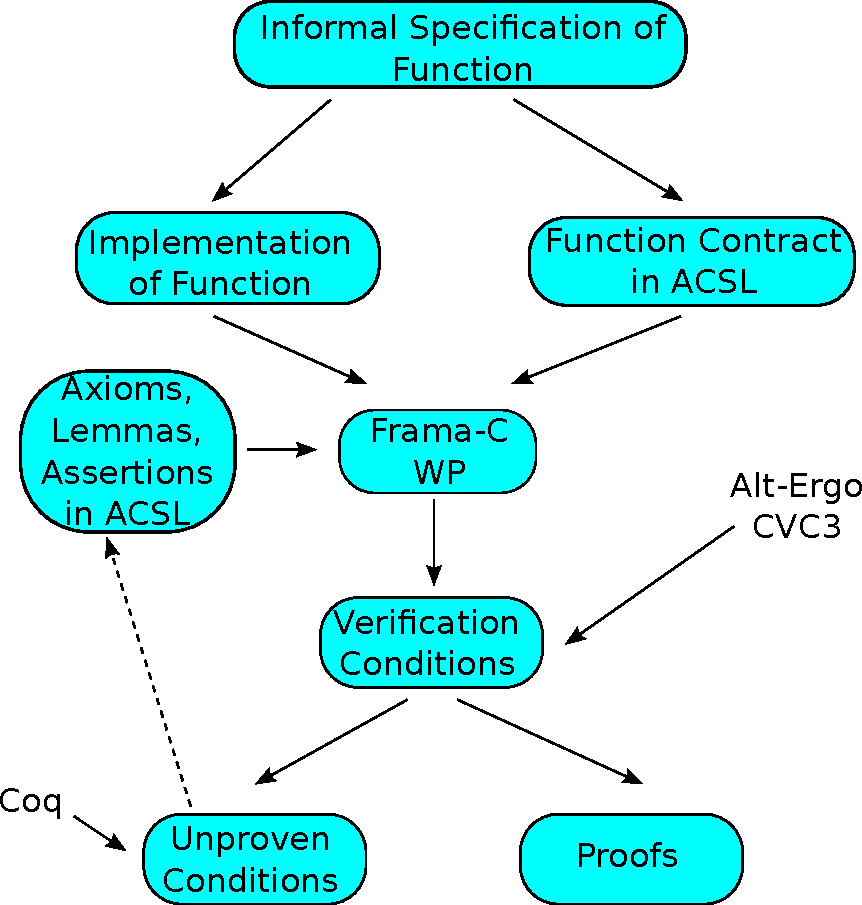
\includegraphics[width=0.60\textwidth]{figures/method-bitwalker.pdf}
\caption{\label{fig:method} The method to formally verify the Bitwalker.}
\end{figure}

Starting point is an informal specification of a function with which in mind
a implementation is written and on which basis the formal specification is created.
The formal specification of a function is a so-called function contract
which contains preconditions to express what a function expects from its caller
and postconditions to state the guarantees after the execution.
The specification language is called 
\acsl (ANSI\slash ISO-\isoc Specification Language)~\cite{acsl} 
which is a formal language to express behavioral properties of \isoc programs.

Moreover, it is the specification language associated with 
the verification platform \framac~\cite{FramaC}
which we use along with its plug-in \wpframac~\cite{wp}.
Within \framac, \wpframac enables the deductive verification of
\isoc programs that have been annotated with \acsl.
\wpframac generates verification conditions which are submitted to external 
automatic or interactive theorem provers.
A function is then verified if each verification condition is discharged
by at least one prover.

Figure~\ref{fig:method} shows that we first apply the automatic
theorem provers \altergo~\cite{alt-ergo} and \cvc~\cite{cvc3}
and then apply the
interactive theorem prover \coq~\cite{Coq}
for the still unproven conditions in order to automate as much as possible.
Moreover, unproven conditions motivate to give some extra information
in the form of axioms, lemmas and assertions in \acsl, 
since they can ease the search of a proof.
One need to be careful with axioms because they can yield contradictions
and thus make the proof system unsound.
This is different for lemmas and assertions
because \wpframac will generate additional verification conditions for them.

In order to prove the absence of run time errors we use
the \inl{rte} option of \wpframac that automatically introduces \acsl
assertions. If all these assertions can be proven, then
the absence of run time errors is guaranteed.


\begin{framed}
The verifiers received the source code without sufficiently clear explanation
about how the inputs and outputs of bitwalker functions are related.
In particular, no information about error conditions were provided.
On such a basis it is, as pointed out on Page~\pageref{lesson},
not possible to write meaningful test cases;
let alone to formally verify the functionality of the bitwalker functions.

In a first step, we therefore inspected the source code and 
derived from this an \emph{informal specification}.
This informal specification is to be understood
as a requirements document for the bitwalker functions as it should have been
available for both the programmer and the verifier.

There are several problems with this approach:
\begin{itemize}
\item
The verifier could make an error while analyzing the source code
and end up with a wrong specification. 
In fact, this happened in a first version.

\item
There could also be an error in the implementation which would then be present also
in the specification, thus leading to the claim ``the code works as implemented''.
\end{itemize}

In order to avoid these problems we submitted our informal specification
for review by the domain experts.
\end{framed}

\clearpage

\subsection{A First Look on \peek and \poke}

In this section we analyse the implementations of \peek 
and \poke.
The goal is to devise a more precise specification than
was original provided.
Of course, a specification derived from the source code by the verifier
must be subject to a review of the domain experts.

At his point we are already using \framacwp in order to identify
potential run time errors in the source code.

\subsubsection{Analysing \peek}

Listing~\ref{lst:peek-original} shows the original implementation of \peek.


\begin{listing}[hbt]
\begin{minipage}{\textwidth}
\lstinputlisting[style=acsl-block, frame=single]{./Bitwalker/Original/Bitwalker_peek.c}
\end{minipage}
\caption{\label{lst:peek-original} Original implementation of \peek}
\end{listing}

Here are some remarks on this implementation.

\begin{itemize}
\item The implementation extensively uses bit operations.
      This is of course largely a matter of taste.
      Nevertheless, it is questionable whether representing a division 
      of an index~\inl{i} by~8 as \inl{i >> 3} is better than writing it as~\inl{i/8}.
\item The argument \inl{Bitstream} represents an array that is only read.
      It is good programming practice to qualify such arguments as \inl{const}.

\item The cast of \inl{CurrentValue != 0} to \inl{uint8_t} is unnecessary for the following reasons:
\begin{itemize}
\item The result of expression \inl{CurrentValue != 0} is of type \inl{int} and has either the value~1 or~0.
\item According to the ``usual arithmetic conversions''\footnote{%
     This is indeed the heading of Section~6.3.1.8 of the C standard.
}
this value will be promoted to the type of \inl{retval << 1} which is~\inl{uint64_t}.
\end{itemize}

    Thus, the cast to \inl{uint8_t} is pointless and removing it increases the clarity of the code.

\end{itemize}

At one point, an alternative to the implementation of \peek in
Listing~\ref{lst:peek-original} was suggested.
This alternative implementation, which is shown in Listing~\ref{lst:peek-alternative}
attempts to limit the use of bit operations to a minimum.


\begin{listing}[hbt]
\begin{minipage}{\textwidth}
\begin{lstlisting}[style=acsl-block,frame=single]
  uint64_t Bitwalker_Peek (unsigned int Startposition,
                           unsigned int Length,
                           uint8_t Bitstream[],
                           unsigned int BitstreamSizeInBytes)
  {
    uint64_t retval = 0;
    for (unsigned int i = Startposition +
           BitstreamSizeInBytes*!((Startposition + Length) <=
           BitstreamSizeInBytes*8);
           i < Startposition + Length; i++)
      retval = (retval*2) +
               (uint8_t)((uint8_t)!!(Bitstream[i/8] & BitwalkerBitMaskTable[i%8]));
    return retval;
 }
\end{lstlisting}
\end{minipage}
\caption{\label{lst:peek-alternative} An alternative implementation of \peek}
\end{listing}

Interestingly, this implementation also employs unnecessary casts to \inl{uint8_t}.
However, the real problem with this alternative implementation is that it produces
different results: Calling \peek from Listing~\ref{lst:peek-original} with the arguments

\begin{verbatim}
  Startposition = 8
  Length = 32
  Bitstream[] = {254, 7, 13, 9}
  BitstreamSizeInBytes = 4
\end{verbatim}

produces~0 whereas the implementation from Listing~\ref{lst:peek-alternative} returns~118294784.
Apparently, even \peek is not so simple that its functionality can be unambiguously
understood just by looking at the code.


\clearpage

Figure~\ref{fig:peek-wp} shows a normalized representation of \peek
that is enhanced with static \acsl assertions.
These assertions can be generated by \framac for all operations where
runtime errors, that is illegal pointer accesses or arithmetic overflows, can occur.
Green bullets indicate potential runtime errors where \framacwp can verify
that they will \emph{not} occur.


\begin{figure}[hbt]
\begin{center}
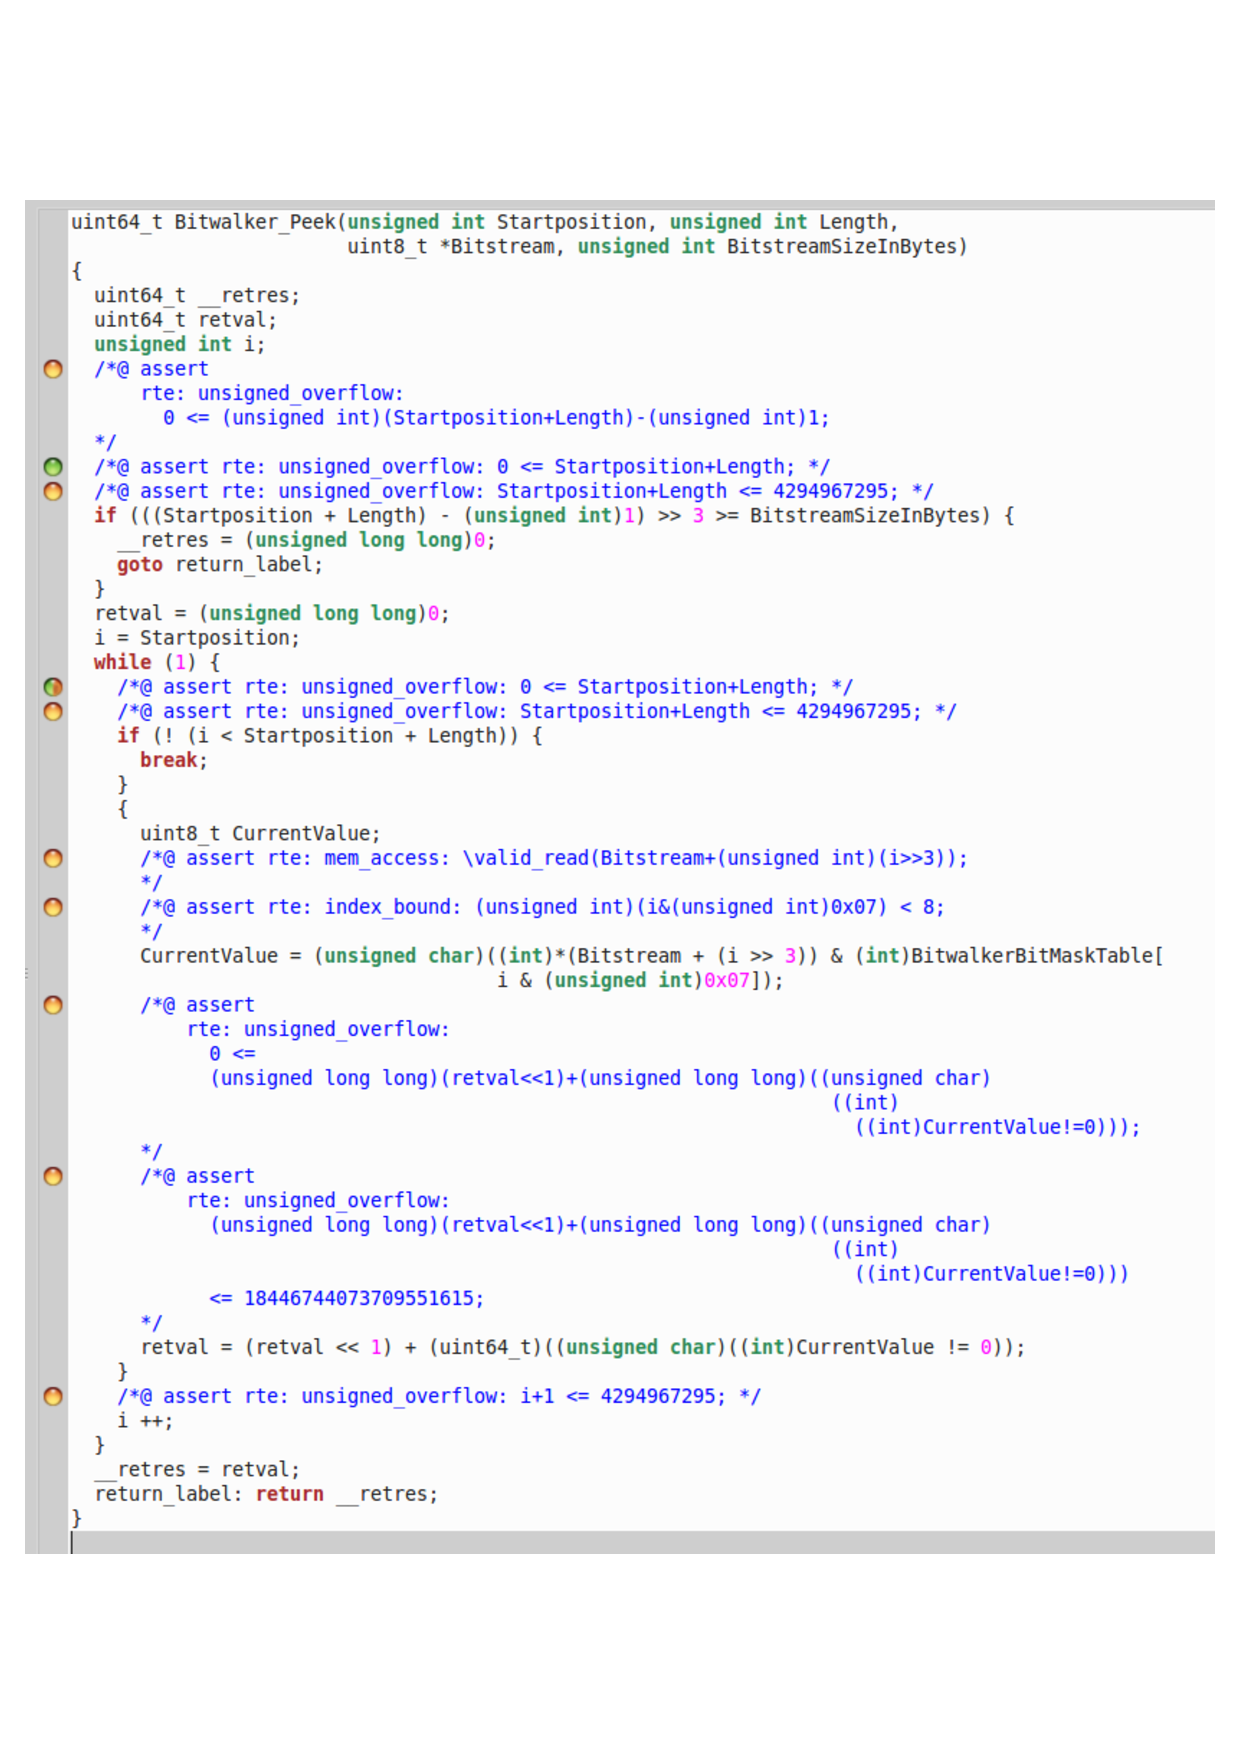
\includegraphics[width=0.95\textwidth]{figures/peek-wp.pdf}
\caption{\label{fig:peek-wp} Potential runtime errors in \peek}
\end{center}
\end{figure}

These potential runtime errors are related to the facts that at this point \framacwp
\begin{itemize}
\item cannot exclude that \inl{Length} can be greater then~64 
\item has to assume that \inl{Startposition + Length} may overflow
\item has no guarantee that \inl{BitstreamSizeInBytes} is the length 
      of the array starting at the address \inl{Bitstream}
\end{itemize}

\clearpage

\subsubsection{Analysing \poke}

Listing~\ref{lst:poke-original} shows the original implementation of \poke.

\begin{listing}[hbt]
\begin{minipage}{\textwidth}
\lstinputlisting[style=acsl-block, frame=single]{./Bitwalker/Original/Bitwalker_poke.c}
\end{minipage}
\caption{\label{lst:poke-original} Original implementation of \poke}
\end{listing}

Clearly visible in the code are various error conditions that are checked 
returned by~\poke.
No specifications for these error conditions have been provided.
 
\clearpage


Figure~\ref{fig:poke-wp} shows the normalized representation of \poke
with \acsl assertions that indicate potential runtime errors.

\begin{figure}[hbt]
\begin{center}
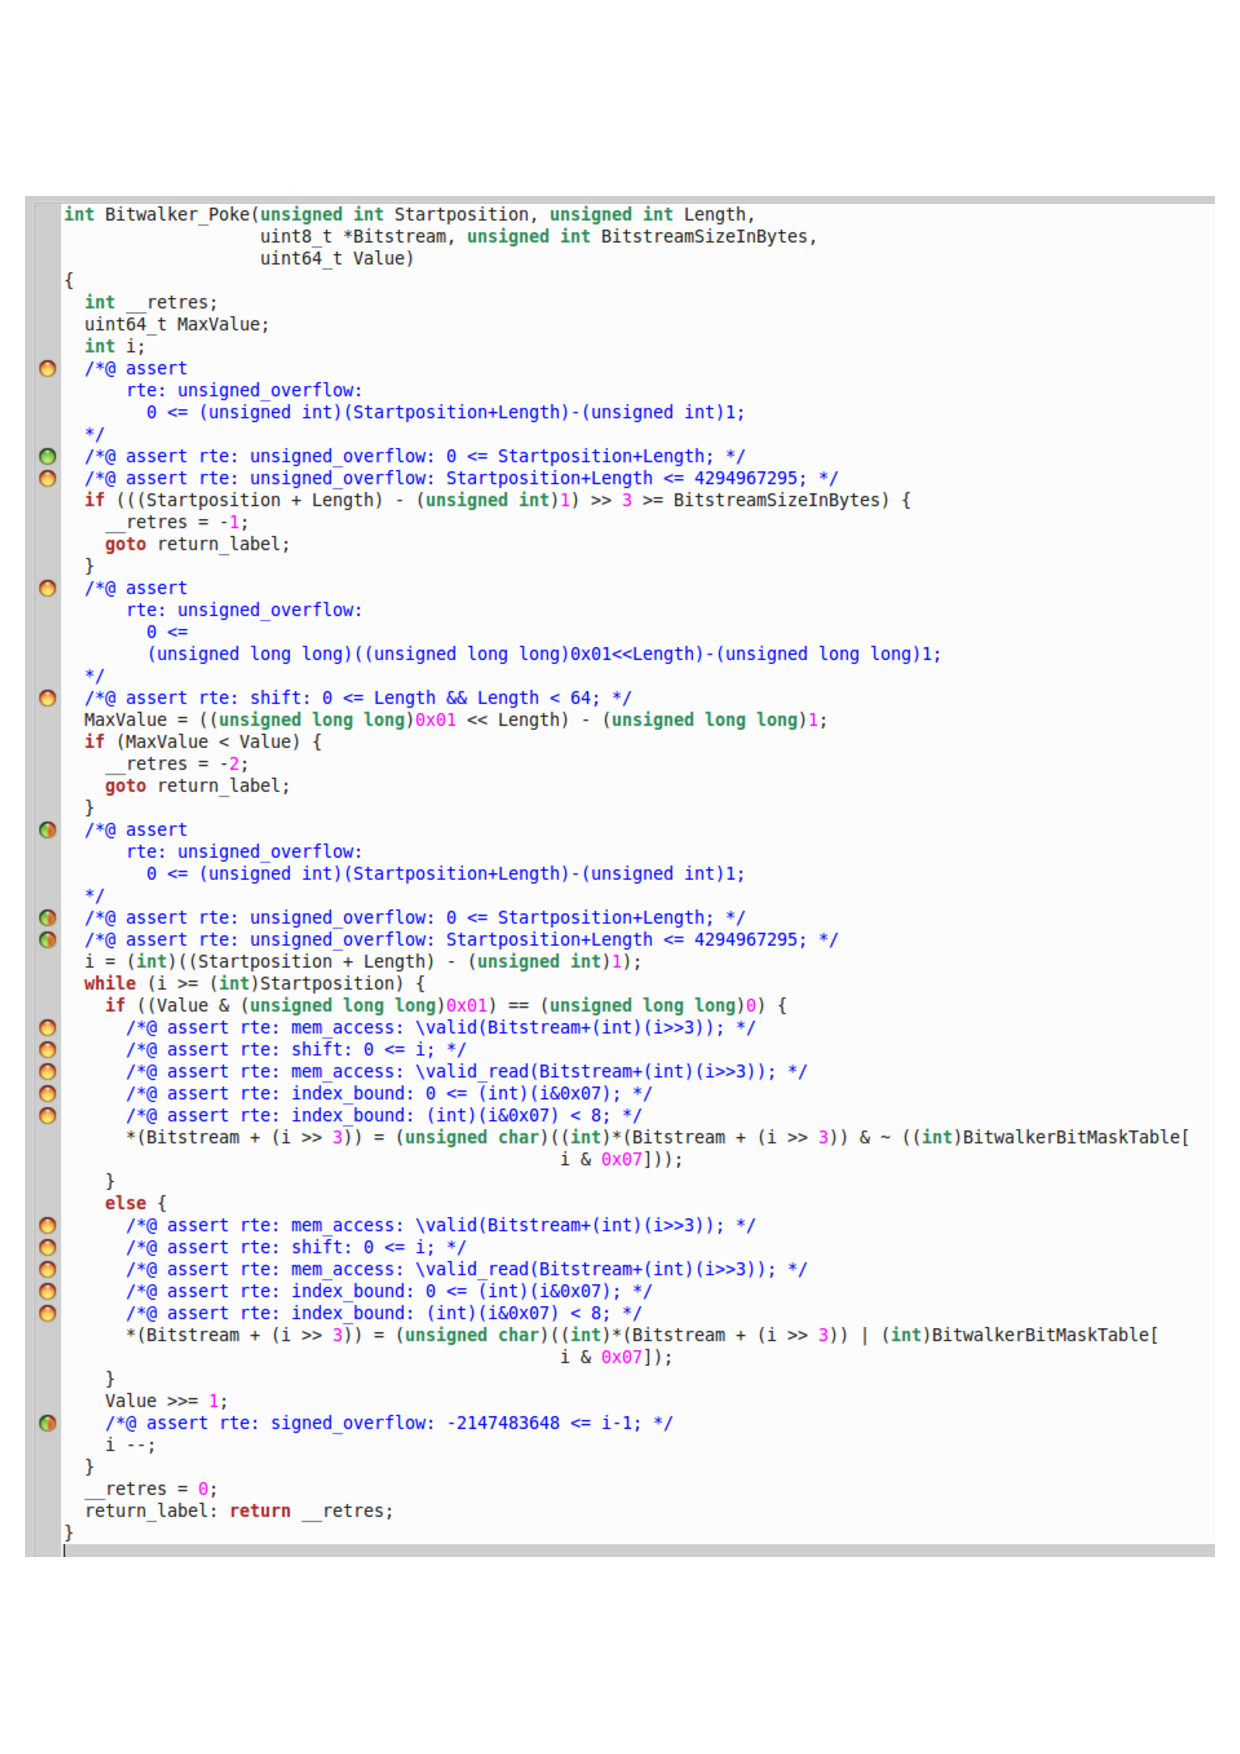
\includegraphics[width=0.99\textwidth]{figures/poke-wp.pdf}
\caption{\label{fig:poke-wp} Potential runtime errors in \peek}
\end{center}
\end{figure}

Similarly to the potential runtime errors of \peek \framacwp
faces the problem that it

\begin{itemize}
\item cannot exclude that \inl{Length} can be greater then~64 
\item has to assume that \inl{Startposition + Length} may overflow
\item has no guarantee that \inl{BitstreamSizeInBytes} is the length 
      of the array starting at the address \inl{Bitstream}
\end{itemize}

\clearpage

\subsection{Informal Specifications}
\label{sec:informal-specification}

Before we provide an informal specification of \peek and \poke, respectively,
we introduce some auxiliary concepts and formulate general assumptions.
We would also like to point out the following: 
When we speak of \emph{integers}, then we refer to the infinite set of mathematical
integers $\{\ldots, -1, 0, 1, \ldots\}$
and not to one of the many finite representation provided by the type system of~C.
This distinction is important because mathematical integers
usually play an important role in \acsl specifications.

\subsubsection{Basic Concepts}

\begin{itemize}
\item
A \emph{bit stream} is an array containing elements of type \verb"uint8_t".

A bit stream of length $n$ contains $8n$ bits.

\item
A bit stream is \emph{valid} if the array is valid.

\item 
A bit stream can be indexed both by its array indices
and its \emph{bit indices}.

Figure~\ref{fig:bitstream-indices} shows the difference between 
array indices and bit indices in a bit stream.
The two bit indices, 0~and~14,
mark bit positions in the first and second array element, respectively.

\begin{figure}[hbt]
\begin{center}
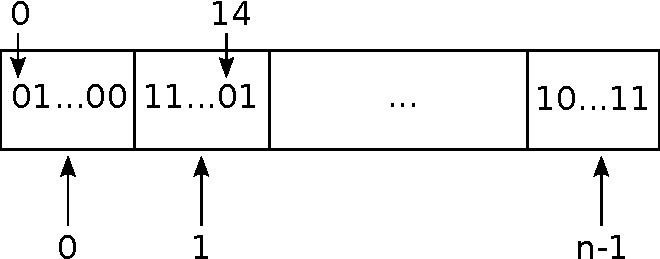
\includegraphics[width=0.40\textwidth]{figures/array_as_stream.pdf}
\caption{\label{fig:bitstream-indices} Array indices and bit indices in a bit stream}
\end{center}
\end{figure}

\item 
The C~programming language neither provides a type \emph{bit}
nor does it support random access to the bits of a bit stream.
In order to access the $i$-th bit of a bit sequence one typically
has to first access the byte with index $j = i/8$ and then access the 
bit $k = i \pmod{8}$ within this byte.
Note that in Figure~\ref{fig:bitstream-indices} 
bytes and bits are indexed in increasing order from the \emph{left}.
On the byte level, however, bits are often indexed from the \emph{right}.
For example, to access the $k$-th bit of a byte \inl{a} one can
shift this bit to the right by $7-k$ and extracts then the now
rightmost bit by performing a bit-wise \emph{and} with the value~1
%
\begin{verbatim}
   (a >> (7-k)) & 1
\end{verbatim}

\item
A \emph{bit sequence} is a consecutive sequence of bits within a bit stream
as represented in Figure~\ref{fig:bitsequence}.
\begin{figure}[hbt]
\begin{center}
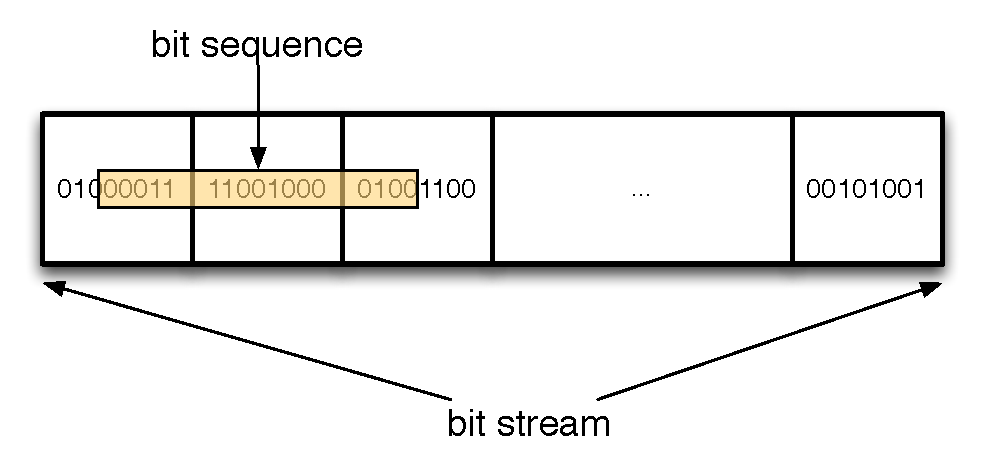
\includegraphics[width=0.40\textwidth]{figures/bit_sequence.pdf}
\caption{\label{fig:bitsequence} A bit sequence within a bit stream}
\end{center}
\end{figure}

A bit sequence is given by the position of its first bit (a bit index in the bit stream)
and its \emph{length}, that is, the number of bits it contains.

\item A bit sequence of length $l$ that starts at bit index $p$ is \emph{valid}
     with respect to a bit stream of length $n$ if the following conditions are
     satisfied
     \begin{align*}
         0 &\leq p < 8n \\
         0 &\leq p + l < 8n
     \end{align*}

\end{itemize}

We assume that the C-types \inl{unsigned int} and \inl{int}, which
are used in the implementation to represent indices, counting and error codes,
have a width of~32~bits.
We point this out here because we conducted the verification on a platform with
these characteristics.

As an aside, MISRA-C discourages the use of ``generic'' integer types
such as \inl{int} and \inl{unsigned int} and recommends the use of integer types whose names
contain the exact width.

\subsubsection{Informal Specification of \peek}
\label{informal-peek}

Now we specify \peek with the introduced auxiliary concepts.
The function \peek reads a bit sequence from a bit stream
and converts it to an integer.

Its function signature reads as follows:

\begin{lstlisting}[style=acsl-block]
uint64_t  Bitwalker_Peek(unsigned int Startposition, 
                         unsigned int Length,
                         uint8_t Bitstream[],
                         unsigned int BitstreamSizeInBytes);
\end{lstlisting}

\paragraph{Arguments}
The arguments of \peek have the following purpose:
\begin{itemize}
    \item \inl{Startposition} is the bit index in the bit stream 
    where the bit sequence starts.
    \item \inl{Length} is the length of the bit sequence.
    \item \inl{Bitstream} is the array which provides the bit stream.
    \item \inl{BitstreamSizeInBytes} is the length of the array 
    containing the bit stream. 
\end{itemize}

\paragraph{Preconditions}
The following preconditions shall hold for the function arguments.
Note that additional constraints are implicitly expressed by the use
of \emph{unsigned} integer types.

\begin{itemize}
\item \inl{Bitstream} is a valid array of length \inl{BitstreamSizeInBytes}

\item \inl{Length} $\leq$ \inl{64} and

\item \inl{Startposition} $\leq$ \inl{UINT_MAX} - \inl{Length}.
      This condition expresses that no arithmetic overflows shall occur
      when evaluating \inl{Startposition + Length}.
\end{itemize}

\paragraph{Description}
As mentioned, the function \peek reads a bit sequence from a bit stream
and converts it to a 64-bit unsigned integer.

For a bit sequence $(b_0, b_1,\ldots,b_{n - 1})$ the function \peek returns the sum
\begin{align}
    \sum_{i=0}^{n-1} b_i \cdot 2^{(n - 1) - i} 
\end{align}

Note that is a higher-level description than what is done in the source code.
There is, in our opinion, not much point to reflect all of the low-level bit operations
into the specification if a clearer description is at hand.

If the bit sequence is not valid, then \peek shall return~0.
We were wondering why the implementation maps an illegal input to a legitimate output.
The code providers argued along the lines that this error condition was not
considered important enough to be properly reported.
One can interpret this design decision as an attempt to increase the
robustness of the function against illegal values.
In general, we recommend to explicitly describe all error conditions
and to devise a consistent error detection and error recovery strategy.


\subsubsection{Informal Specification of \poke}

In this section we examine the function \poke
in the same manner as we did it for \peek.

The function \poke converts an integer to a bit sequence and writes it
into a bit stream.
Its function signature reads as follows:
\begin{lstlisting}[style = acsl-block]
int      Bitwalker_Poke(unsigned int Startposition,
                        unsigned int Length,
                        uint8_t Bitstream[],
                        unsigned int BitstreamSizeInBytes,
                        uint64_t Value);
\end{lstlisting}


\paragraph{Arguments}
The arguments have the following purpose:

\begin{itemize}
    \item \inl{Startposition} is the bit index in the bit stream 
    where the bit sequence starts.
    \item \inl{Length} is the length of the bit sequence.
    \item \inl{Bitstream} is the array which provides the bit stream.
    \item \inl{BitstreamSizeInBytes} is the length of the array 
    containing the bit stream. 
    \item \inl{Value} is the integer which shall be converted into a bit sequence.
\end{itemize}


\paragraph{Preconditions}
The following conditions shall hold for the function arguments:

\begin{itemize}
\item \inl{Bitstream} is a valid array of length \inl{BitstreamSizeInBytes}

\item \inl{Startposition + Length} is less than \verb"UINT_MAX".
\end{itemize}

Note that additional constraints are implicitly expressed by the use
of \emph{unsigned} integer types.


\paragraph{Description}
Now we can specify \poke as follows:
The function \poke converts a 64-bit unsigned integer to a bit sequence and 
writes it into a bit stream.

For $0 \leq x$ exists a shortest sequence of~0 and~1
$(b_0, b_1,\ldots,b_{n - 1})$
such that
\begin{align}
    \sum_{i=0}^{n-1} b_i \cdot 2^{(n - 1) - i} = x.
\end{align}

The function \poke tries to store the sequence $(b_0, b_1,\ldots,b_{n - 1})$
in the bit sequence of \inl{Length} bits that starts
at bit index \inl{Startposition}.

The return value of \poke depends on the following three cases:

\begin{itemize}
\item 
If the bit sequence is valid, then there are two cases:

\begin{itemize}
\item
If \inl{Length} is greater or equal than $n$, then  the sequence
$(\overbrace{0,\ldots,0}^{\mathtt{Length}-n},b_0, b_1,\ldots,b_{n - 1})$
is stored in the bit stream starting at \inl{Startposition}.
The return value of \poke is 0.

\item
If \inl{Length}  is less then $n$, then the
sequence $(b_0, b_1,\ldots,b_{n - 1})$ cannot be stored and\\
\poke returns~$-2$.
\end{itemize}

\item 
If the bit sequence is not valid, then \poke returns~$-1$.
\end{itemize}

\clearpage

\subsection{Tests for \peek and \poke}

In this section we show some tests for \peek and \poke.
These tests were derived from the informal specification in 
Section~\ref{sec:informal-specification}.

We use the \CC\ class \inl{boost::dynamic_bitset} in order to represent
\inl{bit sequences} in our tests.
This class\footnote{
  See \url{http://www.boost.org/doc/libs/1_55_0/libs/dynamic_bitset/dynamic_bitset.html}
},
which is part of the \textsf{Boost} libraries,
provides a higher-level and easier to use interface to bit sequences than is possible in~C.

Specifically, we use in our \CC\ test code the following typedefs

\begin{lstlisting}[style = acsl-block]
  typedef std::vector<uint8_t>           Bytestream;

  typedef boost::dynamic_bitset<uint8_t> Bitstream;
\end{lstlisting}

to represent arrays of sequences of bytes and bits, respectively.
An object of type \inl{Bitstream} can be initialized with an object
of type \inl{Bytestream}. The type \inl{Bitstream} offers random access
to its stored bits.
In addition, it allows to
\begin{itemize}
\item  compute the unsigned value represented in the bit stream by calling the
       method \inl{to_ulong()}, thereby representing the functionality of \peek
\item  create a bit stream from an unsigned integer value by a special constructor,
       thus representing the functionality of \poke
\end{itemize}

Listings~\ref{lst:test_peek} and~\ref{lst:test_poke} show fragments of our test code
for \peek and \poke, respectively.

While testing the Bitwalker was not our main objective it proved useful for
the following reasons.

\begin{itemize}
\item It helped us formulating the formal specifications of \peek and \poke.
  
\item It allowed us to quickly detect that the alternative implementation of
      \peek in Listing~\ref{lst:peek-alternative} is not equivalent to the
      original implementation in Listing~\ref{lst:peek-original}.

\item It provided some assurance that our re-implementations of \peek and \poke
      that we use in Section~\ref{sec:formal-specification} do not behave differently
      than the original implementations.
\end{itemize}

\clearpage

\begin{listing}[hbt]
\begin{minipage}{\textwidth}
\lstinputlisting[style=acsl-block, frame=single]{./Bitwalker/Tests/test_peek.cpp}
\end{minipage}
\caption{\label{lst:test_peek} Test code for \peek}
\end{listing}

\clearpage

\begin{listing}[hbt]
\begin{minipage}{\textwidth}
\lstinputlisting[style=acsl-block, frame=single]{./Bitwalker/Tests/test_poke.cpp}
\end{minipage}
\caption{\label{lst:test_poke} Test code for \poke}
\end{listing}

\clearpage

\subsection{Formal Specification with \acsl}
\label{sec:formal-specification}
\label{formal-peek}

\fxfatal{not ready for review}

In order to verify that the given implementation of \peek fulfills 
the informal specification, we have to formalize the specification.
Listing~\ref{fig:spec-peek} shows such a formalization in \acsl for \peek.

\begin{listing}[hbt]
\begin{minipage}{\textwidth}
\lstinputlisting[style=acsl-block, frame=single]{./Bitwalker/Modified3/Bitwalker_Peek.h}
\end{minipage}
\caption{\label{fig:spec-peek} Formal specification of \peek in \acsl}
\end{listing}

We specify a function contract for \peek containing preconditions
and postconditions introduced by the key words \inl{requires}
and \inl{ensures}, respectively.
In addition, the \acsl language provides the \inl{assigns} clause to specify 
that a function is not allowed to change memory locations other than the ones 
explicitly listed. 
When no \inl{assigns} clauses are specified, 
the function is allowed to modify every accessible memory location. 

The three preconditions for the function arguments of the informal specification 
are formalized straight forward in the function contract also by three preconditions.
For the first one we use the predicate \inl{IsValidRange}
which we specified in \acsl in order to state that the \inl{Bitstream}
is a valid array of length \inl{BitstreamSizeInBytes}.
Furthermore, we claim {\it via} the \inl{assigns} clause 
that \peek does not alter any memory location
apart from local variables.

Moreover, we use so-called behaviors in \acsl for a distinction of the two cases
from the informal specification.
The cases are discriminated through the predicate \inl{ValidBitIndex}
which indicates whether a bit sequence is valid or not.
The first behavior \inl{out\_of\_range} represents the robustness 
case where the bit sequence is not valid and 
the second behavior specifies the expected behavior in the normal case.


Since the implementation of \peek contains a loop,
we need a loop specification containing a variant for the termination
proof and some invariants to enable the automatic theorem provers
to verify the postconditions.
Although this loop specification is important for the verification,
it is not used for formalizing the informal specification.

\begin{listing}[hbt]
\begin{minipage}{\textwidth}
\lstinputlisting[style=acsl-block, frame=single]{./Bitwalker/Modified3/Bitwalker_Peek.c}
\end{minipage}
\caption{\label{fig:spec-peek} Implementation of \peek with \acsl loop invariants}
\end{listing}

Since we verify the implementation with respect to the formal specification, 
it is crucial that it matches the informal one. 
Therefore, we reviewed the accordance of both specifications.

\clearpage

Listing~\ref{lst:spec-poke} shows the function contract of \poke.
The case independent preconditions of the informal specification 
are reflected by the  first three \inl{requires}-clauses at the beginning of the contract.
\poke modifies the \inl{Bitstream} and reads the array
\inl{BitwalkerBitMaskTable} thus we need to express 
that the two arrays must have separated memory locations. 
Therefore, we use the predicate \inl{separated} in the fourth \inl{requires}-clause.
Furthermore, in the following \inl{assigns}-clause we specify the memory locations which 
can be altered by the function.

We specify the three cases of \poke by using behaviors. 
The first behavior \inl{out\_of\_range} occurs if the given bit sequence is not valid with respect to the \inl{Bitstream}. 
The second behavior \inl{value\_too\_big} covers the case where the value \inl{Value} 
is not representable with only \inl{Length} bits.

Finally, the behavior \inl{normal} assumes 
that \inl{Value} is not too big and the bit sequence is valid. 
Here, \poke writes the particular bit sequence into \inl{Bitstream} 
while all other memory locations are unaltered.
For all behaviors there is one postcondition to state what
the return value shall be in this case.


\begin{listing}[hbt]
\begin{minipage}{\textwidth}
\lstinputlisting[style=acsl-block, frame=single]{./Bitwalker/Modified3/Bitwalker_Poke.h}
\end{minipage}
\caption{\label{lst:spec-poke} Formal Specification of \poke}
\end{listing}


\clearpage

\begin{listing}[hbt]
\begin{minipage}{\textwidth}
\lstinputlisting[style=acsl-block, frame=single]{./Bitwalker/Modified3/Bitwalker_Poke.c}
\end{minipage}
\caption{\label{lst:spec-poke} Implementation of \poke with loop invariants}
\end{listing}

\clearpage

\subsection{Formal Verification with \framacwp}
\label{sec:verification}
\label{verification-peek}

\fxfatal{not ready for review}

In this section we present the current state of the verification results 
for \peek.
Table~\ref{tab:results-peek} discriminates the results for
three different types of verification conditions (VCs).

\begin{table}[hbt]
  \centering
  \begin{tabular}[htb]{lccc}
    \toprule
     & \# VC & Proven VCs & Verification rate in \%\\
    \midrule
    lemmas & 1 &0 & 0 \\
    %\midrule
    rte-assertions&9&5&55\\
    rest &18 &17&94\\
 %   \bottomrule
%    &27&22&81\\
    \bottomrule
  \end{tabular}
  \caption{Verification Results of \peek}
  \label{tab:results-peek}
\end{table}


The first row contains the lemmas we used to ease the verification for the automatic theorem provers.
The second row contains the \inl{rte}-assertions 
concerning the absence of run time errors.
The third row shows all other verification conditions for \peek
which are mainly about functional behavior.
However, they also contain the postconditions for the robustness cases
and the loop specification.

For each row we listed the total number of generated verification conditions,
the number of proven verification conditions and the verification rate
that is the percentage of proven verification conditions. 

The verification rate for the \inl{rte}-assertions are very low 
due to the difficulty for \framac to deal with bit operations.
In order to increase this rate, we will verify the absence
of run time errors separately and will provide additional lemmas and axioms
to ease the verification.
We point out some of the related challenges in section~\ref{issues}.



In this section we present the current state of verification results of 
for \poke.
The results are shown in Table~\ref{tab:results-poke}.
 We listed the different verification conditions 
 row by row like we did for \peek.

The function \poke has significantly more unproven verification conditions than \peek
this is because it is more complex and alters memory locations via bit operations.
Therefore, we will verify the absence of run time errors separately as well.

\begin{table}[hbt]
  \centering
  \begin{tabular}[h]{lccc}
    \toprule
     & \# VC & Proven VCs & Proven VCs in \%\\
    \midrule
    lemmas & $1$ &$0$ & $0$ \\
    %\midrule
    rte-assertions&$19$&$7$&$36$\\
    rest &$49$ &$38$&$77$\\
    %\bottomrule
    %&$68$&$45$&$66$\\
    \bottomrule
  \end{tabular}
  \caption{Verification Results of \poke}
  \label{tab:results-poke}
\end{table}

\clearpage

\subsection{Open Issues}
\label{issues}

\fxfatal{not ready for review}


We have seen in this section that \wpframac currently does not deal very well with bit operations.
This is due to the fact that \wpframac's memory models do not provide 
much information about bit operations.
As a consequence, the provers have few options to manipulate the proof goal.
This problem is known and \cealist is working on a solution for the next release of \wpframac.

As a workaround one could introduce axioms which provide
additional facts about bit operations. 
The problem with using axioms is that one can easily introduce wrong facts
which lead to contradictions making the whole proof system unsound. 
Thus, this approach requires a careful review of the added axioms.

Moreover, the chosen automatic theorem provers are generally not very
good when it comes to mixing arithmetic and bit operations.
There is, however, an automatic theorem prover, namely \z,
which can handle arithmetic and bit operations, using a specific syntax.
\framac's interface for \z does not currently takes advantage of this, 
but this may change in a future release.
We therefore expect a better automatic verification rate for the verification of BitWalker.

Another approach to deal with unproven verification conditions consists in
applying an \emph{interactive theorem prover} such as \coq.
Using \coq's rich support for proof manipulation would certainly be very helpful
for the discharge of more proof obligations.

\cleardoublepage

\chapter{Static Analysis of Bitwalker}
\label{sec:static-analysis}

\section{Introduction}
In this chapter we describe our work on the static code analysis of the bitwalker code provided in \href{https://github.com/openETCS/validation/tree/master/Artifacts/Subset-026-7_XML/Subset026_7/Bitwalker}{[validation repository]}

Our aim is to discover programing errors, obtain code metrics (lines of code, lines of code/lines of comments, cyclomatic complexity, Halsted metrics and others) and verify the C11 standard and some subset of rules defined in the MISRA C Standard. That is, we focus on the different aspects of the source code to ensure the quality of the code in various perspectives.

The code metrics help understanding the complexity of the code and can lead to code changes. The complexity metrics allows us to identify particularly complex program areas that it would be desirable to redesign, and where problems that will appear in the maintenance phase are likely focused. For example, the cyclomatic complexity or the number of paths, is a software quality metric that quantifies the complexity of a program and also indicates the number of test cases that would have to be written to execute all paths in a program. However, the cyclomatic complexity only considers the decision structure of a program, and not the complexity of nesting. There are more complexity metrics that takes into account the degree of nesting of a program or that consider the volumen and the program level like the Halstead metrics. The conjunction of the complexity metrics are an important indicator of the code readability, maintainability and portability, and the more complex the code is, the more likely it contains masked bugs.

CENELEC Standard identifies techniques and measures for 5 levels of software safety integrity and requires the use of a package of techniques and their correct
application appropriate to the software safety integrity level.

Six different static analysis tools have been used during the code verification activities in order to assess the quality of the results, ensure code quality and cover different techniques and metrics high recommended by CENELEC Standard. The selected tools are:
\begin{itemize}
\item \textbf{Resource Standard Metrics (\href{http://msquaredtechnologies.com/m2rsm/}{RSM})}: a source code metrics and quality analysis tool
\item \textbf{\href{http://www.locmetrics.com/}{LocMetrics}}: a simple tool for counting lines of code in C\#, Java, and C++
\item \textbf{\href{http://www.scitools.com/}{Understand}}: a reverse engineering, documentation and metrics tool for C and C++ source code. It offers code navigation using a detailed cross reference, a syntax colorizing "smart" editor, and a variety of graphical reverse engineering views.                          
\item \textbf{\href{http://clang-analyzer.llvm.org/}{Clang Static Analyzer}}: The Clang Static Analyzer consists of both a source code analysis framework and a standalone tool that finds bugs in C and Objective-C programs.
\item \textbf{\href{http://cppcheck.sourceforge.net/}{CPPcheck}}: a static analysis tool for C, C++ code. Unlike C, C++ compilers and many other analysis tools it does not detect syntax errors in the code. Cppcheck primarily detects the types of bugs that the compilers normally do not detect. 
\item \textbf{\href{http://www.verifysoft.com/en_cmtx.html}{Testwell CMT++}}: Based on the static properties of the program code CMT++ gives estimates how error prone the program source code is due to its complexity, how long it will take to understand the code, what is the logical volume of the code, etc ...
\end{itemize}


Finally, according to the results obtained by using the tools, we will present some conclusions.

\section{Resource Standard Metrics -RSM- Results}
In this section we provide the results obtained with the \href{http://msquaredtechnologies.com/m2rsm/}{[RSM]} tool.

Resource Standard Metrics (RSM) is a source code metrics and quality analysis tool. This tool provides standard metrics and a combination of features that allow to:
\begin{itemize}
\item Analyze source code for programming errors
\item Analyze source code for code style enforcement
\item Collect Source Code Metrics by the function, class, file, and project
\item Analyze Cyclomatic Complexity
\end{itemize}

Besides, RSM has intrinsic quality notices, can be extended by the end user with User Defined Quality Notices using regular expressions to analyze code lines and it is mapped to the MISRA C Standard. 

RSM has been customized to obtain the below metrics and analysis and the corresponding reports that are available into the \href{https://github.com/openETCS/validation/tree/master/VnVUserStories/VnVUserStorySQS/04-Results}{[VnVUserStories folder]}

\begin{itemize}
\item Project Functional Metrics and Analysis
\item Project Class/Struct Metrics and Analysis
\item Project Quality Profile
\item Quality Notice Density
\item Files Keywords and Metrics
\item Project Keywords and Metrics
\item Files Function Metrics
\item Class/Struct Metrics
\item Complexity Metrics
\end{itemize}

As mentioned previously CENELEC Standard requires the use of a package of techniques. With the use of the RSM tool the following Cenelec Standard techniques have been covered:
\begin{itemize}
\item Limited Size and Complexity in Functions, Subroutines and Methods (High Recommended)
\item Coding Standard (Mandatory): At this point the fulfillment of some of the MISRA-C Standard rules has been checked.
\end{itemize}

\subsection{Quality Metrics}

As well as having intrinsic and user defined quality notices, RSM tool is mapped to the MISRA C Industry Standard. Taking into account the intrisic quality notice and the user defined quality notices the RSM tool covers 40.16\% of \href{http://msquaredtechnologies.com/m2rsm/docs/QualityStandards/MISRA_C_Mapping.htm}{[MISRA C]} rules.

The following table shows the intrinsic Quality Notices for C language that RSM tool checks.

{\footnotesize\sffamily\centering
  \begin{longtable}{||p{.45\textwidth}|p{.5\textwidth}||}
  \caption{Quality Notices}\\
    \hline\hline
    \hline\hline
    \endhead
    \hline\hline
    \endfoot
    \textbf{Quality Notice No. 1}

Emit a quality notice when the physical line length is greater than the specified number of characters.

Rationale:  \textcolor{red}{Reproducing source code on devices that are limited to 80 columns of text can cause the truncation of the line or wrap the line.  Wrapped source lines are difficult to read, thus creating weaker peer reviews of the source code}.
& \textbf{Quality Notice No. 2}

Emit a quality notice when the function name length is greater than the specified number of characters.  

Rationale:  \textcolor{red}{Long function names may be a portability issue especially when code has to be cross compiled onto embedded platforms.  This difficulty is typically seen with older hardware and operating systems.}
    \\
    \hline \textbf{Quality Notice No. 3}
    
Emit a quality notice when ellipsis '...' are identified within a functions parameter list thus enabling variable arguments.  

Rationale:  \textcolor{red}{Ellipsis create a variable argument list.  This type of design is found in C and C++.  It essentially breaks the type strict nature of C++ and should be avoided.}
 & \textbf{Quality Notice No. 4}
 
Emit a quality notice if there exists an assignment
operator '=' within a logical 'if' condition.

Rationale:  \textcolor{red}{An assignment within an "if" condition is likely a typographical error giving rise to a logic defect.  However, some programmers place compound statements into the "if" condition making the code difficult to read.}
    \\
    \hline \textbf{Quality Notice No. 5}
    
Emit a quality notice if there exists an assignment
operator '=' within a logical 'while' condition.

Rationale:  \textcolor{red}{An assignment within a "while" condition is likely a typographical error giving rise to a logic defect.  However, some programmers place compound statements into the "while" condition making the code difficult to read.}
 & \textbf{Quality Notice No. 6}
 
Emit a quality notice when a pre-decrement operator '--' is identified within the code.  

Rationale: \textcolor{red}{ The pre-decrement of a variable occurs before the remainder of the processing in the statement.  This can be difficult to comprehend or anticipate.  There are documented cases where the mathematical results vary between the result of macros when different code preprocessors expand the macros into a normal form.  Remember, there is no standard for the preprocessor, just the language.}
    \\
    \hline \textbf{Quality Notice No. 7}
    
Emit a quality notice when a pre-increment operator '++' is identified within the code.

Rationale:  \textcolor{red}{The pre-increment of a variable occurs before the remainder of the processing in the statement.  This can be difficult to comprehend or anticipate.  There are documented cases where the mathematical results vary between the result of macros when different code preprocessors expand the macros into a normal form.}  
& \textbf{Quality Notice No. 8}

Emit a quality notice when the 'realloc' function
is identified within the code.

Rationale:  \textcolor{red}{Using realloc can lead to latent memory leaks within your C or C++ code.  The call to realloc reassigns the pointer to the same memory address using a larger or smaller space.  However if realloc fails, a NULL pointer is returned.  No "free" was performed on the pointer so if you don't retain the pointer before the realloc call, a latent memory leak could occur.}
    \\
    \hline \textbf{Quality Notice No. 9}
    
Emit a quality notice when the 'goto' function
is identified within the code.

Rationale:  \textcolor{red}{The use of "goto" creates spaghetti code.  A "goto" can jump anywhere to the destination label.  This type of design breaks the "one in - one out" ideal of a function creating code which can be impossible to debug or maintain.}
 & \textbf{Quality Notice No. 10}
 
Emit a quality notice when the Non-ANSI function prototype is identified within the code.

Rationale:  \textcolor{red}{Older C code can be written in a style that does not use function prototypes of the function argument types.  This code will not compile on ANSI C and C++ compilers because of this type of weakness.  Identifying this condition can help assess whether code can be ported to a newer version of the language.}
    \\
    \hline \textbf{Quality Notice No. 11}
    
Emit a quality notice when open and closed brackets '[ ]' are not balanced within a file.

Rationale:  \textcolor{red}{This type of error is always caught by the compiler as a syntax error.  However, a compiler can be told to ignore source code by using preprocessor directives like \#if ... \#endif.  This is a way to "comment" out large blocks of code.  However, the code still looks like operational code to the maintainer as it is not a comment.  Many hours can be wasted working on dead code.  This quality notice serves to warn you of this dead code that should be removed or converted to actual comment form.}
 & \textbf{Quality Notice No. 12}
 
Emit a quality notice when open and closed parentheses '( )' are not balanced within a file.

Rationale:  \textcolor{red}{This type of error is always caught by the compiler as a syntax error.  However, a compiler can be told to ignore source code by using preprocessor directives like \#if ... \#endif.  This is a way to "comment" out large blocks of code.  However, the code still looks like operational code to the maintainer as it is not a comment.  Many hours can be wasted working on dead code.  This quality notice serves to warn you of this dead code that should be removed or converted to actual comment form.}.
    \\
    \hline \textbf{Quality Notice No. 13}
    
Emit a quality notice when a 'switch' statement does not have a 'default' condition.

Rationale:  \textcolor{red}{A "switch" statement must always have a default condition or this logic construct is non-deterministic.  Generally the default condition should warn the user of an anomalous condition which was not anticipated by the programmer by the case clauses of the switch.}
 & \textbf{Quality Notice No. 14}
 
Emit a quality notice when there are more 'case' conditions than 'break', 'return' or 'fall through' comments.

Rationale:  \textcolor{red}{Many tools, including RSM, watch the use of "case" and "break" to ensure that there is not an inadvertent fall through to the next case statement.  RSM requires the programmer to explicitly indicate in the source code via a "fall through" comment that the case was designed to fall through to the next statement.}
    \\
    \hline \textbf{Quality Notice No. 16}
    
Emit a quality notice when function white space
percentage is less than the specified minimum.

Rationale:  \textcolor{red}{Source code must be easily read.  A low percentage of white space indicates that the source code is crammed together thus compromising the readability of the code.  Typically white space less than 10 percent is considered crammed  code. }
 & \textbf{Quality Notice No. 17}
 
Emit a quality notice when function comment
percentage is less than the specified minimum.

Rationale:  \textcolor{red}{A programmer must supply sufficient comments to enable the understandability of the source code.  Typically a comment percentage less than 10 percent is considered insufficient.  However, the content quality of the comment is just as important as the quantity of the comments.  For this reason you could use the -E option to extract all the comments from a file.  The reviewer should be able to read the comments and extract the story of the code.}
    \\
    \hline \textbf{Quality Notice No. 18}
    
Emit a quality notice when the eLOC within a
function exceeds the specified maximum.

Rationale:  \textcolor{red}{An extremely large function is very difficult to maintain and understand.  When a function exceeds 200 eLOC (effective lines of code), it typically indicates that the function could be broken down into several functions.  Small modules are desirable for modular composability.}
 & \textbf{Quality Notice No. 19}
 
Emit a quality notice when file white space
percentage is less than the specified minimum.

Rationale:  \textcolor{red}{Source code must be easily read.  A low percentage of white space indicates that the source code is crammed together thus compromising the readability of the code.  Typically white space less than 10 percent is considered crammed  code.}

    \\
    \hline \textbf{Quality Notice No. 20}
    
Emit a quality notice when file comment
percentage is less than the specified minimum.

Rationale:  \textcolor{red}{A programmer must supply sufficient comments to enable the understandability of the source code.  Typically a comment percentage less than 10 percent is considered insufficient.  However, the content quality of the comment is just as important as the quantity of the comments.  For this reason you could use the -E option to extract all the comments from a file.  The reviewer should be able to read the comments and extract the story of the code.}
 & \textbf{Quality Notice No. 22}
 
Emit a quality notice when each if, else, for
or while is not bound by scope.

Rationale:  \textcolor{red}{Logical blocks should be bound with scope.  This clearly marks the boundaries of scope for the logical blocks.  Many times, code may be added to non-scoped logic blocks thus pushing other lines of code from the active region of the logical construct giving rise to a logic defect.}
    \\
    \hline 
    \textbf{Quality Notice No. 23}
    
Emit a quality notice when the '?' or the implied
if-then-else construct has been identified.

Rationale:  \textcolor{red}{The ? operator creates the code equivalent of an "if" then "else" construct.  However the resultant source is far less readable.}
 & \textbf{Quality Notice No. 24}
 
Emit a quality notice when an ANSI C++ keyword is identified within a *.c or a *.h file.

Rationale: \textcolor{red}{ In C source code it is possible to find variable names like "class".  This word is a key word in C++ and would prevent this C code from being ported to the C++ language.}
    \\
    \hline
\textbf{Quality Notice No. 25} (Deprecated RSM 6.70) 

When analyzing *.h files for C++ keywords,
assume that *.h can be both C and C++.

Rationale: \textcolor{red}{ A *.h file can be either a C or C++ source file.  If a *.h file is assumed to be from either language, then RSM will not emit C keyword notices in *.h file, only for *.c files.}
 & \textbf{Quality Notice No. 26}
 
Emit a quality notice when a void * is identified
within a source file.

Rationale:  \textcolor{red}{A "void *" is a type-less pointer.  ANSI C and C++ strive to be type strict.  In C++ a "void *" breaks the type strict nature of the language which can give rise to anomalous run-time defects.}
    \\
    \hline
    \textbf{Quality Notice No. 27}
    
Emit a quality notice when the number of function return points is greater than the specified maximum.

Rationale:  \textcolor{red}{A well constructed function has one entry point and one exit point.  Functions with multiple return points are difficult to debug and maintain.}
 & \textbf{Quality Notice No. 28}
 
Emit a quality notice when the cyclomatic complexity of a function exceeds the specified maximum.

Rationale:  \textcolor{red}{Cyclomatic complexity is an indicator for the number of logical branches within a function.  A high degree of V(g), greater than 10 or 20, indicates that the function could be broken down into a more modular design of smaller functions.}
    \\
    \hline
        \textbf{Quality Notice No. 29}
        
Emit a quality notice when the number of function input parameters exceeds the specified maximum.

Rationale:  \textcolor{red}{A high number of input parameters to a function indicates poor modular design.  Data should be grouped into representative data types.  Functions should be specific to one purpose.}
 & \textbf{Quality Notice No. 30}
 
Emit a quality notice when a TAB character is identified within the source code. Indentation with TAB will create editor and device dependent formatting.

Rationale:  \textcolor{red}{Tab characters within source code create documents that are print and display device dependent.  The document may look correct on the screen but it may become unreadable when printed.}
    \\
    \hline
        \textbf{Quality Notice No. 31}
        
Emit a quality notice when class comment
percentage is less than the specified minimum.

Rationale:  \textcolor{red}{A programmer must supply sufficient comments to enable the understandability of the source code.  Typically a comment percentage less than 10 percent is considered insufficient.}
 & \textbf{Quality Notice No. 43}
 
Emit a quality notice when the key word 'continue' has been identified within the source code.

Rationale:  \textcolor{red}{The use of 'continue' in logical structures causes a disruption in the linear flow of the logic.  This style of  programming can make maintenance and readability difficult.}
    \\
    \hline
        \textbf{Quality Notice No. 46}
        
Emit a quality notice when function, struct, class or interface blank line percentages are less than the specified minimum
 
Rationale:  \textcolor{red}{The amount of blank lines in a file can indicate the degree of readability in the file. It indicates the author intended his work to be human consumable.}
 & \textbf{Quality Notice No. 47}
 
Emit a quality notice when the file blank line percentage is less than the specified minimum

Rationale: \textcolor{red}{The amount of blank lines in a file can indicate the degree of readability in the file. It indicates the author indented his work to be human consumable.}
    \\
    \hline
        \textbf{Quality Notice No. 48}
        
Emit a quality notice when a function has no logical lines of code. 
 
Rationale: \textcolor{red}{This condition indicates a no-op or stubbed out function with no operational code. Many code generators create such no-op functions which contribute to code bloat and unnecessary resource utilization.}
 & \textbf{Quality Notice No. 49}
 
Emit a quality notice when a function has no parameters in the parameter list.

Rationale:  \textcolor{red}{A function should always specify the actual parameter names to enhance maintenance and readability. A programmer should always put void to indicate the deliberate design in the code.}
    \\
    \hline
        \textbf{Quality Notice No. 50}
         
Emit a quality notice when a variable is assigned to a literal value. Configurable for literal 0 in rsm.cfg. 

Rationale: \textcolor{red}{A symbolic constant is the preferred method for variable assignment as this creates maintainable and understandable code.}
 & \textbf{Quality Notice No. 51}
 
Emit a quality notice when there is no comment before a function block. 
 
Rationale: \textcolor{red}{A function block should retain a preceding comment block describing the purpose, parameters, returns and algorithms.}
    \\
    \hline
     \textbf{Quality Notice No. 52}
     
Emit a quality notice when there is no comment before a class block. 
 
Rationale: \textcolor{red}{A class block should retain a preceding comment block describing the purpose, and algorithms.}
 & \textbf{Quality Notice No. 53}
 
Emit a quality notice when there is no comment before a struct block. 

Rationale: \textcolor{red}{A struct block should retain a preceding comment block describing the data and purpose.}
    \\
    \hline
     \textbf{Quality Notice No. 55}
     
Emit a quality notice when scope exceeds the specified maximum in the rsm.cfg file. 
 
Rationale: \textcolor{red}{A deep scope block of complex logic or levels may indicate a maintenance concern.}
 & \textbf{Quality Notice No. 56}
 
Emit a quality notice when sequential break statements are identified.

Rationale: \textcolor{red}{Repetitive and sequential breaks can be used to fool RSM identification of case statement without breaks.}
    \\
    \hline
\end{longtable}}

In addition to this, some user defined quality notices are included in the rsm\_udqn.cfg file. The table below shows those that are active and defined for C language.

{\footnotesize\sffamily\centering
  \begin{longtable}{||p{.45\textwidth}|p{.5\textwidth}||}
  \caption{User Defined Quality Notices}\\
    \hline\hline
    \hline\hline
    \endhead
    \hline\hline
    \endfoot
    \textbf{User Defined Quality Notice No. 102}

Emit a quality notice when dynamic memory using malloc is not initialized.
& \textbf{User Defined Quality Notice No. 103}

Emit a quality notice when the realloc function has been identified.  
    \\
    \hline \textbf{User Defined Quality Notice No. 104}
    
Emit a quality notice when a line containing just a semicolon has been identified.  
& \textbf{User Defined Quality Notice No. 105}
 
Emit a quality notice when a symbolic constant using \#define has been identified
    \\
    \hline \textbf{User Defined Quality Notice No. 107}
    
Emit a quality notice when a double ;; has been identified.  
& \textbf{User Defined Quality Notice No. 109}
 
Emit a quality notice when a double pointer indirection has been identified
    \\
    \hline \textbf{User Defined Quality Notice No. 116}
    
Emit a quality notice if Pointer variable uninitialized.  
& \textbf{User Defined Quality Notice No. 125}
 
Emit a quality notice when a data member in the header file is not of the form m\_*
    \\
    \hline
\end{longtable}}

Taking into account the quality notices mentioned above, a table that indicates the total quality profile (Summary by notice type) for the bitwalker code is shown. This result is especially useful for determining the overall internal code quality.
           
\begin{longtable}{||p{.1\textwidth}|p{.1\textwidth}|p{.1\textwidth}|p{.6\textwidth}||}
  \caption{Quality Profile}\\
    \hline\hline
    \textbf{Type} & \textbf{Count} & \textbf{Percent} & \textbf{Quality Notice} \\
    \hline\hline
    \endhead
    \hline\hline
    \endfoot
    \textcolor{red}{1} & \textcolor{blue}{38}
& 9.57
& Physical line length > 80 characters
    \\
    \hline
    \textcolor{red}{2} & \textcolor{blue}{4}
& 1.01
& Function name length > 32 characters
    \\
    \hline
    \textcolor{red}{22} & \textcolor{blue}{5}
& 1.26
& if, else, for or while not bound by scope
    \\
    \hline
    \textcolor{red}{27} & \textcolor{blue}{2}
& 0.50
& Number of function return points > 1
    \\
    \hline
    \textcolor{red}{30} & \textcolor{blue}{330}
& 83.12
& TAB character has been identified
    \\
    \hline
    \textcolor{red}{50} & \textcolor{blue}{7}
& 1.76
& Variable assignment to a literal number
    \\
    \hline
    \textcolor{red}{51} & \textcolor{blue}{8}
& 2.02
& No comment preceding a function block
    \\
    \hline
    \textcolor{red}{53} & \textcolor{blue}{1}
& 0.25
& No comment preceding a struct block
    \\
    \hline
    \textcolor{red}{125} & \textcolor{blue}{2}
& 0.50
& A data member in the header file is not of the form m\_*
    \\
    \hline
\end{longtable}

More detailed information regarding to in what line, function or file the quality notices have been detected is provided in the \href{https://github.com/openETCS/validation/blob/master/VnVUserStories/VnVUserStorySQS/04-Results/bitwalker_functional_quality_metrics.htm}{[bitwalker\_functional\_quality\_metrics file]}. 

\subsection{Complexity Metrics}
Reflecting on elements that can contribute to increase the complexity of a program and influencing in its maintenance, four elements are identified:
\begin{itemize}
\item Program Size
\item Data Structure
\item Data Flow
\item Control Flow
\end{itemize}

\subsubsection{Program Size Metrics}
\label{sec:sizem}
Very large programs are complex even if only be for the large amount of information to be considered in order to understand them. So a first measure of the code complexity is given by its size. This size can be determined using the following metrics:
\begin{itemize}
\item Number of lines
\item Halstead metrics (See \ref{sec:halsted})
\end{itemize}

Counting the number of code lines in a program is a simple way to measure its size. The main problem with this metric is to decide what we consider as line.
The reason is that there is no standard definition of what a line of code is. Do comments count? Are data declarations included? What happens if a statement extends over several lines? – These are the questions that often arise. According to the criteria that we follow a different metric will be obtained.

For example, in C language, a line of code can be:
\begin{itemize}
\item a statement, instruction finished in a jump line
\item a statement, instruction terminated with a semi-colon
\item any line of the program terminated with a new line (comments included)
\end{itemize}

As there is no standard definition and the definitions of these metrics are tied to specific computer languages, a definition of how the RSM tool considers these code metrics is indicated below.

\begin{itemize}
\item An effective line of code is the measurement of all lines that are not comments, blanks or standalone braces or parenthesis. RSM counts the instances of lines that contain a single brace and parenthesis and creates a metric for effective lines of source code, eLOC. This metric is the result of subtracting the single braces and parenthesis from the LOC measurement.
\item Logical lines of code represent a metrics for those line of code which form code statements. These statements are terminated with a semi-colon. The control line for the "for" loop contain two semi-colons but accounts for only one semi colon.
\item Comments: RSM counts a comment line as any physical line that contains a comment.
\end{itemize}

Taking into account these criterias the following size metrics are obtained:

\begin{longtable}{||p{.275\textwidth}|p{.125\textwidth}|p{.125\textwidth}|p{.125\textwidth}|p{.125\textwidth}||}
  \caption{File Summary}\\
    \hline\hline
    \textbf{Metrics} & \textbf{Bitwalker.h} & \textbf{Bitwalker.c} & \textbf{opnETCS.h} & \textbf{opnETCS \_Decoder.h}\\
    \hline\hline
    \endhead
    \hline\hline
    \endfoot
    \ LOC\footnote{Lines of Code}. & 15
& 58
& 884 & 62
    \\
    \hline
    \ eLOC\footnote{Effective Lines of Codes} & 15
& 40
& 823 & 62
    \\
    \hline
    \ lLOC\footnote{Logical Statements Lines of Code: represent a metrics for those line of code which form code statements.  These statements are terminated with a semi-colon.  The control line for the "for" loop contain two semi-colons but accounts for only one semi colon} & 11
& 28
& 760 & 61
    \\
    \hline
    \ Comment & 16
& 29
& 822 & 15
    \\
    \hline
    \ Lines & 41
& 109
& 1249 & 84
    \\
    \hline
   \end{longtable}

The following table describes some recommendations for the lines-of-code measures:

\clearpage

\begin{longtable}{||p{.175\textwidth}|p{.175\textwidth}|p{.675\textwidth}||}
    \caption{\label{lst:recom} Recommendations}\\
    \hline\hline
    \textbf{Measures} & \textbf{Values} & \textbf{Comments}\\
    \hline\hline
    \endhead
    \hline\hline
    \endfoot
    \ Function length & 4-40 program lines
& A function definition contains at least a prototype, one line of code, and a pair of braces, which makes 4 lines.

A function longer than 40 program lines probably implements many functions. Functions containing one selection statement with many branches are an exception to this rule.

Decomposing them into smaler functions often decreases readability.
    \\
    \hline
    \ File length & 4-400 program lines
& The smallest entity that may reasonably occupy a whole source file is a function, and the minimum length of a function is 4 lines. Files longer than 400 program lines (10..40 functions) are usually too long to be understood as a whole.
    \\
    \hline
    \ Comments Percentage & 30\%-75\%
& If less than one third of a file is comments the file is either very trivial or poorly explained.

If more than 75\% of a file are comments, the file is not a program but a document.
In a well-documented header file percentage of comments may sometimes exceed 75\%
    \\
    \hline
   \end{longtable}

By analyzing the results, one can observe the Bitwalker.c file fulfills the recommendations in relation to the file length. Although the comments percentage (26\%) is a little bite under the recommended value, this do not indicate a poor documentation of source code.

\subsubsection{Control Flow Metrics}
\label{sec:cyclo}
The possibility that the execution flow of a program follows different paths depending on whether or not certain conditions are met, increases the difficulty to understand what the program do in each of the situations that may occur.

One metric that addresses the complexity of the control flow is the \textbf{Cyclomatic complexity}. 

The cyclomatic complexity metric measures the complexity of the code by counting the number of independent paths through a piece of code-by counting the number of decision points. The decision point is where a choice can be made during execution; this gives rise to different paths through the code. Decision points arise through if statements and through while, do while and for loops. A single switch or try statement can also add many more decision points. This metric can either be determined by counting the regions, nodes and edges or number of predicate nodes (branching points) with a flow graph.


The following equations defined McCabe Cyclomatic Complexity: 
\begin{itemize}
\item The number of regions in a flow graph.
\item V(g) = E - N + 2P, where E are the edges, N are the nodes and P nodes without outgoing path.
\item V(g) = P + n, where P are the predicate nodes and n the number of output.
\end{itemize}

When the graph is strongly connected, a simplified formula to compute the cyclomatic complexity is use: V(g) = P + 1, where P are the predicate nodes.

The result obtained in the calculation of the cyclomatic complexity also determines the upper bound on the number of tests that must be performed to ensure that each statement is executed at least once.

At following the results of some complexity metrics obtained by the RSM tool are shown:

\begin{longtable}{||p{.275\textwidth}|p{.125\textwidth}|p{.125\textwidth}|p{.075\textwidth}|p{.125\textwidth}|p{.125\textwidth}||}
  \caption{Functional Summary}\\
    \hline\hline
    \textbf{Metrics} & \textbf{Bitwalker.c}\\
    \hline\hline
    \endhead
    \hline\hline
    \endfoot
    \ File Function Count
& 7
    \\
    \hline
    \ Total Function LOC
& 49
    \\
    \hline
    \ Total Function eLOC
& 31
    \\
    \hline
    \ Total Function lLOC
& 27
    \\
    \hline
    \ Total Function Params
& 20
    \\
    \hline
    \ Total Cyclo Complexity
& 13
    \\
    \hline
    \ Total Function Pts LOC
& 0.5
    \\
    \hline
    \ Total Function Pts eLOC
& 0.3
    \\
    \hline
    \ Total Function Pts lLOC
& 0.2
    \\
    \hline
    \ Total Function Return
& 10
    \\
    \hline
    \ Total Function Complex
& 43
    \\
    \hline
    \ Max Function LOC
& 16
    \\
    \hline
    \ Max Function eLOC
& 12
    \\
    \hline
    \ Max Function lLOC
& 9
    \\
    \hline
    \ Average Function LOC
& 7.00
    \\
    \hline
    \ Average Function eLOC
& 4.43
    \\
    \hline
    \ Average Function lLOC
& 3.86
    \\
    \hline
    \ Max Function Parameters
& 5
    \\
    \hline
    \ Max Function Returns
& 3
    \\
    \hline
    \ Max Interface Complex
& 8
    \\
    \hline
    \ Max Cyclomatic Complex
& 5
    \\
    \hline
    \ Max Total Complexity
& 13
    \\
    \hline
    \ Avg Function Parameters
& 2.86
    \\
    \hline
    \ Avg Function Returns
& 1.43
    \\
    \hline
    \ Avg Interface Complex
& 4.29
    \\
    \hline
    \ Avg Cyclomatic Complex
& 1.86
    \\
    \hline
    \ Avg Total Complexity
& 6.14
    \\
    \hline
\end{longtable}

The interface complexity is defined by RSM as the number of input parameters to a function plus the number of return states from that function. Class interface complexity is the sum of all function interface complexity metrics within that class.

The Maximun total complexity is the addition of Maximun Interface and Cyclomatic complexities and the total Cyclomatic complexity is calculated as the sum of the cyclomatic complexity of each function of the file. 

Knowing that a program has a high value of cyclomatic complexity (total Cyclomatic complexity) does not provide us enough info to decide what actions to take to improve our software. This occurs because there is not an approximate threshold reference value for total cyclomatic complexity since not all software has the same size. However we can say that the cyclomatic complexity of each function should not exceed a certain value.

Due to this, a more detailed Complexity analysis per function is provided at following.

\begin{longtable}{||p{.125\textwidth}|p{.125\textwidth}|p{.175\textwidth}|p{.175\textwidth}||}
  \caption{Function Metrics}\\
    \hline\hline
    \endhead
    \hline\hline
    \endfoot
\multicolumn{4}{||l||}{\textbf{Bitwalker\_Peek}}
\\\hline
\multicolumn{4}{||l||}{Cyclomatic Complexity Vg Detail:}
\\\hline
\multicolumn{3}{||c|}{Function Base} & 1
\\\hline
\multicolumn{3}{||c|}{Loops for / foreach} & 1
\\\hline
\multicolumn{3}{||c|}{Conditional if / else if} & 1
\\\hline
\ Param: 4 &
Return: 2 &
Cyclo Vg: 3 &
Comment: 5
 \\\hline
\ LOC: 12 &
eLOC: 8 &
lLOC: 7 &
Lines: 19
 \\\hline
\multicolumn{4}{||l||}{\textbf{Bitwalker\_Poke}}
\\\hline
\multicolumn{4}{||l||}{Cyclomatic Complexity Vg Detail:}
\\\hline
\multicolumn{3}{||c|}{Function Base} & 1
\\\hline
\multicolumn{3}{||c|}{Loops for / foreach} & 1
\\\hline
\multicolumn{3}{||c|}{Conditional if / else if} & 3
\\\hline
\ Param: 5 &
Return: 3 &
Cyclo Vg: 5 &
Comment: 6
 \\\hline
\ LOC: 16 &
eLOC: 12 &
lLOC: 9 &
Lines: 23
 \\\hline
\multicolumn{4}{||l||}{\textbf{Bitwalker\_IncrementalWalker\_Init}}
\\\hline
\ Param: 4 &
Return: 1 &
Cyclo Vg: 1 &
Comment: 0
 \\\hline
\ LOC: 5 &
eLOC: 3 &
lLOC: 3 &
Lines: 5
 \\\hline
\multicolumn{4}{||l||}{\textbf{Bitwalker\_IncrementalWalker\_Peek\_Next}}
\\\hline
\ Param: 2 &
Return: 1 &
Cyclo Vg: 1 &
Comment: 1
 \\\hline
\ LOC: 5 &
eLOC: 3 &
lLOC: 3 &
Lines: 6
 \\\hline
\multicolumn{4}{||l||}{\textbf{Bitwalker\_IncrementalWalker\_Peek\_Finish}}
\\\hline
\ Param: 1 &
Return: 1 &
Cyclo Vg: 1 &
Comment: 0
 \\\hline
\ LOC: 3 &
eLOC: 1 &
lLOC: 1 &
Lines: 3
 \\\hline
\multicolumn{4}{||l||}{\textbf{Bitwalker\_IncrementalWalker\_Poke\_Next}}
\\\hline
\ Param: 3 &
Return: 1 &
Cyclo Vg: 1 &
Comment: 1
 \\\hline
\ LOC: 5 &
eLOC: 3 &
lLOC: 3 &
Lines: 6
 \\\hline
\multicolumn{4}{||l||}{\textbf{Bitwalker\_IncrementalWalker\_Poke\_Finish}}
\\\hline
\ Param: 1 &
Return: 1 &
Cyclo Vg: 1 &
Comment: 0
 \\\hline
\ LOC: 3 &
eLOC: 1 &
lLOC: 1 &
Lines: 3
 \\\hline
\end{longtable}

After calculating the cyclomatic complexity the risk involved can be determined using the following table:

{\footnotesize\sffamily\centering
  \begin{longtable}{||p{.15\textwidth}|p{.40\textwidth}||}
  \caption{Mc Cabe cyclomatic Complexity Reference table}\\
    \hline\hline
    \textbf{Cyclomatic Complexity} & \textbf{Risk Evaluation} \\
    \hline\hline
    \endhead
    \hline\hline
    \endfoot
    \textbf{1-10}
& Low risk
    \\
    \hline
    \textbf{11-20}
& More complex, Moderate risk
    \\
    \hline
    \textbf{21-50}
& Complex, High Risk
    \\
    \hline
    \textbf{>50}
& Not testable, Very High Risk
    \\
    \hline
\end{longtable}}

If we cross the values ​​obtained in the analysis with the indicative table we can see that all functions are under 10, so we speak of simple functions with little logic and with low risk.

According to Cenelec the modular approach involves several rules for the design, code and maintenance phases. As a result, an appropriate restriction must be specified for the total number of parameters, which are usually 5. Bearing this in mind, the table presented above shows that this is fulfilled for each function.

Furthermore, from the previous definition of recommended values for lines of code measures (see \ref{lst:recom}), we can see there is not documentation for some functions.

Now, an example of the cyclomatic complexity calculation for the bitwalker\_Poke function is shown to compare the correctness of these results .

\begin{listing}[hbt]
\begin{minipage}{\textwidth}
\lstinputlisting[style=acsl-block, frame=single]{./figures/poke.impl}
\end{minipage}
\caption{Bitwalker\_Poke}
\end{listing}

The control flow generated from the bitwalker\_Poke function would look like figure 4.1.

\begin{figure}[H]
\centering
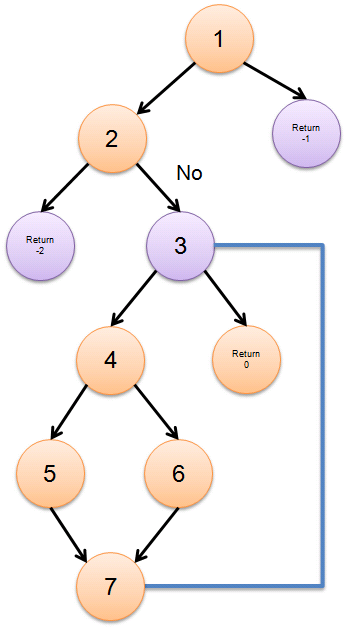
\includegraphics[width=0.45\textwidth]{./figures/flow.png}
\caption{Bitwalker\_Poke Flow}
\end{figure}

In this flow, 4 predicated nodes are displayed so, taking into account the equation V(g) = P + 1, where P are the predicate nodes, we see that the cyclomatic complexity of this function is V(g)=5.

\section{LocMetrics tool Results}

\href{http://www.locmetrics.com/}{[LocMetrics]} tool counts total lines of code (LOC), blank lines of code (BLOC), comment lines of code (CLOC), lines with both code and comments (C\&SLOC), logical source lines of code (SLOC-L), McCabe VG complexity (MVG), Header Comments (HCLOC), Header Words (HCWORD) and number of comment words (CWORDS). Physical executable source lines of code (SLOC-P) is calculated as the total lines of source code minus blank lines and comment lines. Counts are calculated on a per file basis and accumulated for the entire project. LocMetrics also generates a comment word histogram.

The results obtained by LocMetrics tool are the following:

\begin{longtable}{||p{.125\textwidth}|p{.055\textwidth}|p{.065\textwidth}|p{.065\textwidth}|p{.055\textwidth}|p{.060\textwidth}|p{.09\textwidth}|p{.065\textwidth}|p{.085\textwidth}|p{.075\textwidth}|p{.1\textwidth}||}
  \caption{LocMetrics Tool Results}\\
    \hline\hline
    \textbf{File} & LOC &  SLOC-P & SLOC-L & MVG & BLOC & C\&SLOC & CLOC & CWORD & HCLOC & HCWORD \\
    \hline\hline
    \endhead
    \hline\hline
    \endfoot
    Bitwalker.h &
    42 & 15 & 12 & 0 & 8 & 1 & 19 & 102 & 0 & 0
    \\
    \hline
    Bitwalker.c &
    110 & 58 & 36 & 15 & 24 & 5 & 28 & 217 & 0 & 0
    \\
    \hline
    opnETCS.h &
    1250 & 884 & 883 & 0 & 181 & 637 & 185 & 3864 & 0 & 0
    \\
    \hline
    opnETCS
    \_Decoder.h &
    85 & 62 & 61 & 0 & 3 & 0 & 20 & 103 & 0 & 0
    \\
    \hline
\end{longtable}

\section{Understand tool Results}
\href{http://www.scitools.com/}{[Understand]} is a cross-platform, multi-language, maintenance-oriented IDE (Interactive Development Environment). It is designed to help maintain and understand large amounts of legacy or newly created source code. 
Understand also provides a way to check the code using coding Standard to avoid potential errors. With this tool SQS has checked MISRA-C:2004 and code metrics (lines of code, complexity, object cross reference, invocation tree, Unused Items and others). The highly recommended and mandatory techniques identified by CENELEC Standard covered by the tool are:
\begin{itemize}
\item Coding Standard (Mandatory)
\item Limited Size and Complexity in Functions, Subroutines and Methods (Highly Recommended)
\item Data Flow Analysis technique (Highly Recommended)
\item Control Flow Analysis technique (Highly Recommended)
\end{itemize}

The detailed static analysis report is available in the \href{https://github.com/openETCS/validation/tree/master/VnVUserStories/VnVUserStorySQS/04-Results}{[VnVUserStories folder]}

Below the \underline{MISRA-C tested rules} are listed:
\begin{itemize}
\item \textbf{Language extensions}
\begin{itemize}
\item 2.1 (req): Assembly language shall be encapsulated and isolated.
\item 2.2 (req): Source code shall only use \inl{/* ... */} style comments.
\item 2.3 (req): The character sequence \inl{/*} shall not be used within a comment.
\item 2.4 (adv-): Sections of code should not be 'commented out'.
\end{itemize}
\item \textbf{Character sets}
\begin{itemize}
\item 4.1 (req): Only those escape sequences that are defined in the ISO C standard shall be used.
\item 4.2 (req): Trigraphs shall not be used.
\end{itemize}
\item \textbf{Identifiers}
\begin{itemize}
\item 5.1 (req): Identifiers (internal and external) shall not rely on the significance of more than 31 characters.
\item 5.2 (req): Identifiers in an inner scope shall not use the same name as an identifier in an outer scope, and therefore hide that identifier.
\item 5.3 (req-): A \inl{typedef} name shall be a unique identifier.
\item 5.4 (req): A tag name shall be a unique identifier.
\item 5.5 (adv-): No object or function identifier with static storage duration should be reused.
\item 5.7 (adv-): No identifier name should be reused.
\end{itemize}
\item \textbf{Types}
\begin{itemize}
\item 6.3 (adv): \inl{typedef}s that indicate size and signedness should be used in place of the basic types.
\item 6.4 (req): Bit fields shall only be defined to be of type \inl{unsigned int} or \inl{signed int}.
\item 6.5 (req-): Bit fields of type signed int shall be at least 2 bits long.
\end{itemize}
\item \textbf{Constants}
\begin{itemize}
\item 7.1 (req): Octal constants (other than zero) and octal escape sequences shall not be used.
\end{itemize}
\item \textbf{Declarations and definitions}
\begin{itemize}
\item 8.5 (req-): There shall be no definitions of objects or functions in a header file.
\item 8.6 (adv): Functions shall be declared at file scope.
\item 8.7 (req): Objects shall be defined at block scope if they are only accessed from within a single function.
\item 8.8 (req): An external object or function shall be declared in one and only one file.
\item 8.9 (req): An identifier with external linkage shall have exactly one external definition.
\item 8.10 (req): All declarations and definitions of objects or functions at file scope shall have internal linkage unless external linkage is required.
\item 8.11 (req): The static storage class specifier shall be used in definitions and declarations of objects and functions that have internal linkage.
\end{itemize}
\item \textbf{Initialisation}
\begin{itemize}
\item 9.3 (req): In an enumerator list, the \inl{=} construct shall not be used to explicitly initialise members other than the first, unless all items are explicitly initialised.
\end{itemize}
\item \textbf{Control statement expressions}
\begin{itemize}
\item 13.3 (req): Floating-point expressions shall not be tested for equality or inequality.
\end{itemize}
\item \textbf{Control flow}
\begin{itemize}
\item 14.1 (req-): There shall be no unreachable code.
\item 14.3 (req-): Before preprocessing, a null statement shall only occur on a line by itself; it may be followed by a comment provided that the first character following the null statement is a white-space character.
\item 14.4 (req): The \inl{goto} statement shall not be used.
\item 14.5 (req): The \inl{continue} statement shall not be used.
\item 14.7 (req): A function shall have a single point of exit at the end of the function.
\item 14.10 (req): All \inl{if ... else if} constructs shall be terminated with an 'else' clause.
\end{itemize}
\item \textbf{Switch statements}
\begin{itemize}
\item 15.3 (req): The final clause of a \inl{switch} statement shall be the 
\inl{default} clause.
\end{itemize}
\item \textbf{Functions}
\begin{itemize}
\item 16.1 (req): Functions shall not be defined with variable numbers of arguments.
\item 16.2 (req): Functions shall not call themselves, either directly or indirectly.
\item 16.3 (req): Identifiers shall be given for all of the parameters in a function prototype declaration.
\item 16.4 (req-): The identifiers used in the declaration and definition of a function shall be identical.
\item 16.5 (req): Functions with no parameters shall be declared with parameter type void.
\end{itemize}
\item \textbf{Pointers and arrays}
\begin{itemize}
\item 17.5 (adv): The declaration of objects should contain no more than 2 levels of pointer indirection.
\end{itemize}
\item \textbf{Structures and unions}
\begin{itemize}
\item 18.4 (req): Unions shall not be used.
\end{itemize}
\item \textbf{Preprocessing directives}
\begin{itemize}
\item 19.1 (adv-): \inl{#include} statements in a file should only be preceded by other preprocessor directives or comments.
\item 19.2 (adv): Non-standard characters should not occur in header file names in include directives.
\item 19.3 (req): The \inl{#include} directive shall be followed by either a \inl{<filename>} or a \inl{<filename>} sequence.
\item 19.4 (req-): C macros shall only expand to a braced initializer, a constant, a parenthesised expression, a type qualifier, a storage class specifier, or a do-while-zero construct.
\item 19.5 (req): Macros shall not be \inl{#define}d or \inl{#undef}d within a block.
\item 19.6 (req): \inl{#undef} shall not be used.
\end{itemize}
\item \textbf{Standard libraries}
\begin{itemize}
\item 20.4 (req): Dynamic heap memory allocation shall not be used.
\item 20.5 (req): The error indicator \inl{errno} shall not be used.
\item 20.6 (req): The macro \inl{offsetof}, in library \inl{<stddef.h>}, shall not be used.
\item 20.7 (req): The \inl{setjmp} macro and the \inl{longjmp} function shall not be used.
\item 20.8 (req): The signal handling facilities of \inl{<signal.h>} shall not be used.
\item 20.9 (req): The input/output library \inl{<stdio.h>} shall not be used in production code.
\item 20.10 (req): The library functions \inl{atof}, \inl{atoi} and \inl{atol} from library \inl{<stdlib.h>} shall not be used.
\item 20.11 (req): The library functions \inl{abort}, \inl{exit}, \inl{getenv} and \inl{system} from library \inl{<stdlib.h>} shall not be used.
\item 20.12 (req): The time handling functions of library \inl{<time.h>} shall not be used.
\end{itemize}
\item \textbf{Run-time failures}
\begin{itemize}
\item 21.1 (req-): Minimization of run-time failures shall be ensured by the use of at least one of: 
\begin{itemize}
\item static analysis tools/techniques;
\item dynamic analysis tools/techniques;
\item explicit coding of checks to handle run-time faults.
\end{itemize}
\end{itemize}
\end{itemize}
 
After a review of the subset of MISRA-C rules taking into account project requirements and sector standard or best practices it is necessary to decide which of them are not to be implemented/approved due to its application can get worse understandability of the code and which other rules of other standard will be applied.

The table below shows the non approved MISRA-C rules.

{\footnotesize\sffamily\centering
  \begin{longtable}{||p{.15\textwidth}|p{.15\textwidth}||}
  \caption{Status of MISRA Rules}\\
    \hline\hline
    \textbf{MISRA Rule} & \textbf{Status} \\
    \hline\hline
    \endhead
    \hline\hline
    \endfoot
    \textbf{Global 5.1}
& no recommended
    \\
    \hline
    \textbf{Global 5.6}
& no recommended
    \\
    \hline
\end{longtable}}


The results of the MISRA Rules are the following:
\begin{figure}[H]
\centering
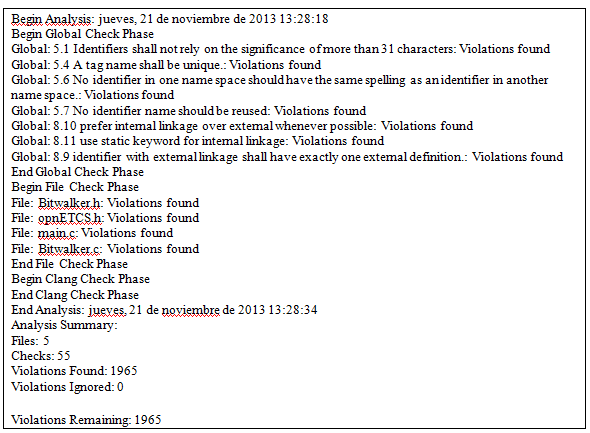
\includegraphics{./figures/understand.png}
\caption{MISRA-C Rules results}
\end{figure}

The files into the violations are found are listed in the below table.

{\footnotesize\sffamily\centering
  \begin{longtable}{||p{.15\textwidth}|p{.8\textwidth}||}
  \caption{Summary of detected MISRA Violations}\\
    \hline\hline
    \textbf{MISRA Rule} & \textbf{Files} \\
    \hline\hline
    \endhead
    \hline\hline
    \endfoot
    \textbf{Global 5.1}
& Bitwalker.c/opnETCS.h/opnETCS\_Decoder.h
    \\
    \hline
    \textbf{Global 5.4}
& opnETCS.h
    \\
    \hline
    \textbf{Global 5.6}
& Bitwalker.c/Bitwalker.h
    \\
    \hline
    \textbf{Global 5.7}
& Bitwalker.c/Bitwalker.h/opnETCS.h
    \\
    \hline
    \textbf{Global 8.9}
& opnETCS\_Decoder.h
    \\
    \hline
    \textbf{Global 8.10}
& main.c
    \\
    \hline
    \textbf{Global 8.11}
& main.c
    \\
    \hline
\end{longtable}}

A detailed information about the file, entity, line, check, etc of all violations detected above can be found in the index files of \href{https://github.com/openETCS/validation/blob/master/VnVUserStories/VnVUserStorySQS/04-Results/results}{[Results]} and \href{https://github.com/openETCS/validation/blob/master/VnVUserStories/VnVUserStorySQS/04-Results/results2}{[Results2]} folders.

In addition to the MISRA-C compliance checking, we also run code metrics analysis in order to ensure the correctness of the obtained results through the results comparation.

Below tables shows some different metrics per file and function.
In order to understand the tables and to be able to compare the results obtained with the different tools the definition of the specific metrics is provided before the presentation of the corresponding table.
\begin{itemize}
\item Cyclomatic: The measure of the complexity of a function's decision structure. The cyclomatic complexity is also the number of basis, or independent, paths through a module. 
\item Modified Cyclomatic: cyclomatic except each case statement is not counted; the entire switch counts as 1.
\item Strict: Cyclomatic complexity except each short-circuit operator adds 1 to the complexity.
\item Essential Complexity: cyclomatic complexity after structured programming constructs have been removed.
\item Nesting: maximum nesting level of control constucts (if, while,etc.)
\item Count Path: Number of unique paths through a body of code (not counting gotos or abnormal exits
\end{itemize}


\begin{longtable}{||p{.275\textwidth}|p{.0025\textwidth}||}
  \caption{Function Complexity metrics}\\
    \hline\hline
    \endhead
    \hline\hline
    \endfoot
\multicolumn{2}{||l||}{\textbf{Bitwalker\_Peek}}
\\\hline
\ Cyclomatic: & 3
\\\hline
\ Modified Cyclomatic: & 3
\\\hline
\ Strict Cyclomatic: & 3
\\\hline
\ Essential: & 1
 \\\hline
\ Max Nesting:   & 1
 \\\hline
\ Count Path: & 3
\\\hline
\multicolumn{2}{||l||}{\textbf{Bitwalker\_Poke}}
\\\hline
\ Cyclomatic: & 5
\\\hline
\ Modified Cyclomatic: & 5
\\\hline
\ Strict Cyclomatic: & 5
\\\hline
\ Essential: & 3
 \\\hline
\ Max Nesting:   & 2
 \\\hline
\ Count Path: & 5
\\\hline
\multicolumn{2}{||l||}{\textbf{Bitwalker\_IncrementalWalker\_Init}}
\\\hline
\ Cyclomatic: & 1
\\\hline
\ Modified Cyclomatic: & 1
\\\hline
\ Strict Cyclomatic: & 1 
\\\hline
\ Essential: & 1
 \\\hline
\ Max Nesting:   & 0
 \\\hline
\ Count Path: & 1
\\\hline
\multicolumn{2}{||l||}{\textbf{Bitwalker\_IncrementalWalker\_Peek\_Next}}
\\\hline
\ Cyclomatic: & 1
\\\hline
\ Modified Cyclomatic: & 1
\\\hline
\ Strict Cyclomatic: & 1 
\\\hline
\ Essential: & 1
 \\\hline
\ Max Nesting:   & 0
 \\\hline
\ Count Path: & 1
\\\hline
\multicolumn{2}{||l||}{\textbf{Bitwalker\_IncrementalWalker\_Peek\_Finish}}
\\\hline
\ Cyclomatic: & 1
\\\hline
\ Modified Cyclomatic: & 1
\\\hline
\ Strict Cyclomatic: & 1 
\\\hline
\ Essential: & 1
 \\\hline
\ Max Nesting:   & 0
 \\\hline
\ Count Path: & 1
\\\hline
\multicolumn{2}{||l||}{\textbf{Bitwalker\_IncrementalWalker\_Poke\_Next}}
\\\hline
\ Cyclomatic: & 1
\\\hline
\ Modified Cyclomatic: & 1
\\\hline
\ Strict Cyclomatic: & 1 
\\\hline
\ Essential: & 1
 \\\hline
\ Max Nesting:   & 0
 \\\hline
\ Count Path: & 1
\\\hline
\multicolumn{2}{||l||}{\textbf{Bitwalker\_IncrementalWalker\_Poke\_Finish}}
\\\hline
\ Cyclomatic: & 1
\\\hline
\ Modified Cyclomatic: & 1
\\\hline
\ Strict Cyclomatic: & 1 
\\\hline
\ Essential: & 1
 \\\hline
\ Max Nesting:   & 0
 \\\hline
\ Count Path: & 1
\\\hline
\end{longtable}

Here are some remarks about how the Understand tool defines and take into account the following code metrics:
\begin{itemize}
\item Lines: total lines (in a function or file or project)
\item Comment Lines: total lines that have comments on them
\item Blank Lines: total lines without any code/comment
\item Code Lines: total lines that have any code on them
\item Executable Lines: total lines that have executable code on them
\item Declarative Lines: total lines that have declarative code on them
\item Execution Statements: total statements in executable code
\item Declaration Statements: total statements in declarative code
\item Ratio Comment/Code: comment lines / code lines
\end{itemize}

\begin{longtable}{||p{.275\textwidth}|p{.125\textwidth}|p{.125\textwidth}|p{.125\textwidth}|p{.125\textwidth}|p{.125\textwidth}||}
  \caption{File Metrics}\\
    \hline\hline
    \textbf{Metrics} & \textbf{Bitwalker.h} & \textbf{Bitwalker.c} & \textbf{opnETCS.h} & \textbf{opnETCS \_Decoder.h}\\
    \hline\hline
    \endhead
    \hline\hline
    \endfoot
    \ Lines: & 41
& 109
& 1249 & 84
    \\
    \hline
    \ Comment Lines: & 20
& 33
& 822 & 20
    \\
    \hline
    \ Blank Lines: & 7
& 23
& 180 & 2
    \\
    \hline
    \ Preprocessor Lines: & 4
& 1
& 1 & 1
    \\
    \hline
    \ Code Lines:  & 11
& 57
& 883 & 61
    \\
    \hline
    \ Inactive Lines:  & 0
& 0
& 0 & 0
    \\
    \hline
    \ Executable Code Lines:  & 0
& 30
& 0 & 0
    \\
    \hline
    \ Declarative Code Lines:  & 11
& 15
& 822 & 61
    \\
    \hline
    \ Execution Statements:  & 0
& 28
& 0 & 0
    \\
    \hline
    \ Declaration Statements:  & 11
& 15
& 760 & 61
    \\
    \hline
    \ Ratio Comment/Code:  & 1.82
& 0.58
& 0.93 & 0.33
    \\
    \hline
    \ Units  & 0
& 7
& 0 & 0
    \\
    \hline
   \end{longtable}
   

\begin{longtable}{||p{.350\textwidth}|p{.0125\textwidth}||}
  \caption{Function code Metrics}\\
    \hline\hline
    \endhead
    \hline\hline
    \endfoot
    \multicolumn{2}{||l||}{\textbf{Bitwalker\_IncrementalWalker\_Init}}
\\\hline
    \ Lines: & 6
    \\
    \hline
    \ Comment Lines: & 0
    \\
    \hline
    \ Blank Lines: & 0
    \\
    \hline
    \ Code Lines:  & 6
    \\
    \hline
    \ Inactive Lines:  & 0
    \\
    \hline
    \ Executable Code Lines:  & 3
    \\
    \hline
    \ Declarative Code Lines:  & 1
    \\
    \hline
    \ Execution Statements:  & 3
    \\
    \hline
    \ Declaration Statements:  & 0
    \\
    \hline
    \ Ratio Comment/Code:  & 0.00
    \\
    \hline
    \multicolumn{2}{||l||}{\textbf{Bitwalker\_IncrementalWalker\_Peek\_Finish}}
\\\hline
    \ Lines: & 4
    \\
    \hline
    \ Comment Lines: & 0
    \\
    \hline
    \ Blank Lines: & 0
    \\
    \hline
    \ Code Lines:  & 4
    \\
    \hline
    \ Inactive Lines:  & 0
    \\
    \hline
    \ Executable Code Lines:  & 1
    \\
    \hline
    \ Declarative Code Lines:  & 1
    \\
    \hline
    \ Execution Statements:  & 1
    \\
    \hline
    \ Declaration Statements:  & 0
    \\
    \hline
    \ Ratio Comment/Code:  & 0.00
    \\
    \hline
    \multicolumn{2}{||l||}{\textbf{Bitwalker\_IncrementalWalker\_Peek\_Next}}
\\\hline
    \ Lines: & 7
    \\
    \hline
    \ Comment Lines: & 1
    \\
    \hline
    \ Blank Lines: & 0
    \\
    \hline
    \ Code Lines:  & 6
    \\
    \hline
    \ Inactive Lines:  & 0
    \\
    \hline
    \ Executable Code Lines:  & 3
    \\
    \hline
    \ Declarative Code Lines:  & 2
    \\
    \hline
    \ Execution Statements:  & 2
    \\
    \hline
    \ Declaration Statements:  & 1
    \\
    \hline
    \ Ratio Comment/Code:  & 0.17
    \\
    \hline
    \multicolumn{2}{||l||}{\textbf{Bitwalker\_IncrementalWalker\_Poke\_Finish}}
\\\hline
    \ Lines: & 4
    \\
    \hline
    \ Comment Lines: & 0
    \\
    \hline
    \ Blank Lines: & 0
    \\
    \hline
    \ Code Lines:  & 4
    \\
    \hline
    \ Inactive Lines:  & 0
    \\
    \hline
    \ Executable Code Lines:  & 1
    \\
    \hline
    \ Declarative Code Lines:  & 1
    \\
    \hline
    \ Execution Statements:  & 1
    \\
    \hline
    \ Declaration Statements:  & 0
    \\
    \hline
    \ Ratio Comment/Code:  & 0.00
    \\
    \hline
    \multicolumn{2}{||l||}{\textbf{Bitwalker\_IncrementalWalker\_Poke\_Next}}
\\\hline
    \ Lines: & 7
    \\
    \hline
    \ Comment Lines: & 1
    \\
    \hline
    \ Blank Lines: & 0
    \\
    \hline
    \ Code Lines:  & 6
    \\
    \hline
    \ Inactive Lines:  & 0
    \\
    \hline
    \ Executable Code Lines:  & 3
    \\
    \hline
    \ Declarative Code Lines:  & 2
    \\
    \hline
    \ Execution Statements:  & 2
    \\
    \hline
    \ Declaration Statements:  & 1
    \\
    \hline
    \ Ratio Comment/Code:  & 0.17
    \\
    \hline
    \multicolumn{2}{||l||}{\textbf{Bitwalker\_Peek}}
\\\hline
    \ Lines: & 20
    \\
    \hline
    \ Comment Lines: & 5
    \\
    \hline
    \ Blank Lines: & 4
    \\
    \hline
    \ Code Lines:  & 13
    \\
    \hline
    \ Inactive Lines:  & 0
    \\
    \hline
    \ Executable Code Lines:  & 7
    \\
    \hline
    \ Declarative Code Lines:  & 4
    \\
    \hline
    \ Execution Statements:  & 7
    \\
    \hline
    \ Declaration Statements:  & 3
    \\
    \hline
    \ Ratio Comment/Code:  & 0.38
    \\
    \hline
        \multicolumn{2}{||l||}{\textbf{Bitwalker\_Poke}}
\\\hline
    \ Lines: & 24
    \\
    \hline
    \ Comment Lines: & 6
    \\
    \hline
    \ Blank Lines: & 4
    \\
    \hline
    \ Code Lines:  & 17
    \\
    \hline
    \ Inactive Lines:  & 0
    \\
    \hline
    \ Executable Code Lines:  & 11
    \\
    \hline
    \ Declarative Code Lines:  & 3
    \\
    \hline
    \ Execution Statements:  & 12
    \\
    \hline
    \ Declaration Statements:  & 2
    \\
    \hline
    \ Ratio Comment/Code:  & 0.35
    \\
    \hline
   \end{longtable}

Taking into account control flow and data flow techniques some Uninitialized Items (items such as variables that are not initialized in the code), Unused Variables and Parameters items (items that are declared (and perhaps initialized) but never referenced other than that) and Unused Program Units have been identified. The Unused Program Units Report identifies program units that are declared but never used. However note that this listing in this report doesnt mean the system doesnt need this program unit.

{\footnotesize\sffamily\centering
  \begin{longtable}{||p{.15\textwidth}|p{.40\textwidth}|p{.15\textwidth}|p{.15\textwidth}||}
  \caption{Unused Variables and Parameters}\\
    \hline\hline
    \textbf{File} & \textbf{Item} & \textbf{Type of Item} & \textbf{Location} \\
    \hline\hline
    \endhead
    \hline\hline
    \endfoot
    \textbf{Bitwalker.c}
& Bitwalker\_IncrementalWalker\_Peek\_Finish & Function & line 91
    \\
    \hline
    \textbf{Bitwalker.c}
& Bitwalker\_IncrementalWalker\_Peek\_Next & Function & line 82
    \\
    \hline
    \textbf{Bitwalker.c}
& Bitwalker\_IncrementalWalker\_Poke\_Finish & Function & line 106
    \\
    \hline
\end{longtable}}

{\footnotesize\sffamily\centering
  \begin{longtable}{||p{.15\textwidth}|p{.15\textwidth}|p{.15\textwidth}||}
  \caption{Uninitialized Items}\\
    \hline\hline
    \textbf{File} & \textbf{Item} & \textbf{Location} \\
    \hline\hline
    \endhead
    \hline\hline
    \endfoot
    \textbf{Bitwalker.c}
& i & line 35
    \\
    \hline
    \textbf{Bitwalker.c}
& i & line 60
    \\
    \hline
\end{longtable}}

{\footnotesize\sffamily\centering
  \begin{longtable}{||p{.15\textwidth}|p{.40\textwidth}|p{.15\textwidth}||}
  \caption{Unused Program Units}\\
    \hline\hline
    \textbf{File} & \textbf{Item} & \textbf{Location} \\
    \hline\hline
    \endhead
    \hline\hline
    \endfoot
    \textbf{Bitwalker.c}
& Bitwalker\_IncrementalWalker\_Peek\_Finish & line 91
    \\
    \hline
    \textbf{Bitwalker.c}
& Bitwalker\_IncrementalWalker\_Peek\_Next & line 82
    \\
    \hline
    \textbf{Bitwalker.c}
& Bitwalker\_IncrementalWalker\_Poke\_Finish & line 106
    \\
    \hline
\end{longtable}}

\section{Clang Static Analyzer tool Results}
The \href{http://clang-analyzer.llvm.org/}{[Clang Static Analyzer]} is a source code analysis tool that finds bugs in C, C++, and Objective-C programs.

The analyzer is 100\% open source and is part of the Clang project. Like the rest of Clang, the analyzer is implemented as a C++ library that can be used by other tools and applications.

With this analysis SQS has checked the following:

{\footnotesize\sffamily\centering
  \begin{longtable}{||p{.45\textwidth}|p{.5\textwidth}||}
  \caption{Aspects checked}\\
    \hline\hline
    \hline\hline
    \endhead
    \hline\hline
    \endfoot
    \textbf{core.AdjustedReturnValue}
& Check to see if the return value of a function call is different than the caller expects (e.g., from calls through function pointers).
    \\
    \hline
    \textbf{core.CallAndMessage}
& Check for logical errors for function calls and Objective-C message expressions (e.g., uninitialized arguments, null function pointers).
    \\
    \hline
    \textbf{core.DivideZero}
& Check for division by zero.
    \\
    \hline
    \textbf{core.NonNullParamChecker}
& Check for null pointers passed as arguments to a function whose arguments are known to be non-null.
    \\
    \hline
    \textbf{core.NullDereference}
& Check for dereferences of null pointers.
    \\
    \hline
    \textbf{core.StackAddressEscape}
& Check that addresses to stack memory do not escape the function.
    \\
    \hline
    \textbf{core.UndefinedBinaryOperatorResult}
& Check for undefined results of binary operators.
    \\
    \hline
    \textbf{core.VLASize}
& Check for declarations of VLA of undefined or zero size.
    \\
    \hline
    \textbf{core.builtin.BuiltinFunctions}
& Evaluate compiler built-in functions (e.g., alloca()).
    \\
    \hline
    \textbf{core.builtin.NoReturnFunctions}
& Evaluate "panic" functions that are known to not return to the caller.
    \\
    \hline
    \textbf{core.uninitialized.ArraySubscript}
& Check for uninitialized values used as array subscripts.
    \\
    \hline
    \textbf{core.uninitialized.Assign}
& Check for assigning uninitialized values.
    \\
    \hline
    \textbf{core.uninitialized.Branch}
& Check for uninitialized values used as branch conditions.
    \\
    \hline
    \textbf{core.uninitialized.CapturedBlockVariable}
& Check for blocks that capture uninitialized values.
    \\
    \hline
    \textbf{core.uninitialized.UndefReturn}
& Check for uninitialized values being returned to the caller.
    \\
    \hline
    \textbf{deadcode.DeadStores}
& Check for values stored to variables that are never read afterwards.
    \\
    \hline
    \textbf{security.FloatLoopCounter}
& Warn on using a floating point value as a loop counter (CERT: FLP30-C, FLP30-CPP).
    \\
    \hline
    \textbf{security.insecureAPI.UncheckedReturn}
& Warn on uses of functions whose return values must be always checked.
    \\
    \hline
    \textbf{security.insecureAPI.getpw}
& Warn on uses of the 'getpw' function.
    \\
    \hline
    \textbf{security.insecureAPI.gets}
& Warn on uses of the 'gets' function.
    \\
    \hline
    \textbf{security.insecureAPI.mkstemp}
& Warn when 'mkstemp' is passed fewer than 6 X's in the format string.
    \\
    \hline
    \textbf{security.insecureAPI.mktemp}
& Warn on uses of the 'mktemp' function.
    \\
    \hline
    \textbf{security.insecureAPI.rand}
& Warn on uses of the 'rand', 'random', and related functions.
    \\
    \hline
    \textbf{security.insecureAPI.strcpy}
& Warn on uses of the 'strcpy' and 'strcat' functions.
    \\
    \hline
    \textbf{security.insecureAPI.vfork}
& Warn on uses of the 'vfork' function.
    \\
    \hline
    \textbf{unix.API}
& Check calls to various UNIX/Posix functions.
    \\
    \hline
    \textbf{unix.Malloc}
& Check for memory leaks, double free, and use-after-free problems involving malloc.
    \\
    \hline
    \textbf{unix.MallocSizeof}
& Check for dubious malloc arguments involving sizeof.
    \\
    \hline
    \textbf{unix.MismatchedDeallocator}
& Check for mismatched deallocators (e.g. passing a pointer allocating with new to free()).
    \\
    \hline
    \textbf{unix.cstring.BadSizeArg}
& Check the size argument passed into C string functions for common erroneous patterns.
    \\
    \hline
    \textbf{unix.cstring.NullArg}
& Check for null pointers being passed as arguments to C string functions.
    \\
    \hline
\end{longtable}}

Taking into account the features checked by the tool, the following Cenelec Standard techniques have been covered:
\begin{itemize}
\item Boundary Value Analysis (High Recommended)
\item Data Flow Analysis (High Recommended)
\end{itemize}

After run this analysis no violation has been found.

\begin{figure}[H]
\centering
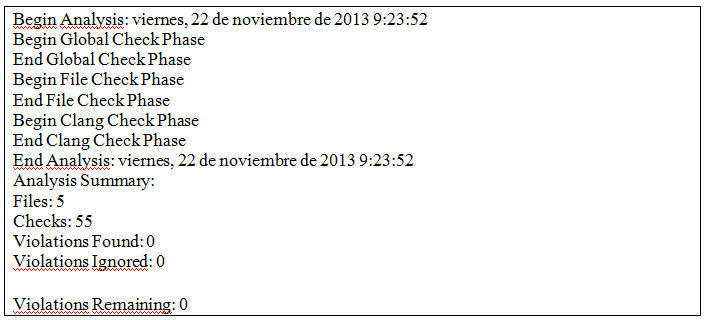
\includegraphics[scale=0.8]{./figures/clang.png}
\caption{Clang Analysis results}
\end{figure}

\section{CPPcheck tool Results}

Bitwalker folder has been analyzed statically by \href{http://cppcheck.sourceforge.net/}{[CPPcheck]} tool (Complying with the standard C11).

Cppcheck supports the following languages: C89, C99, C11 and a wide variety of static checks. The following features are provided:
\begin{itemize}
\item Out of bounds checking
\item Check the code for each class
\item Checking exception safety
\item Memory leaks checking
\item Warn if obsolete functions are used
\item Check for uninitialized variables and unused functions
\item Check input/output operations
\item Null pointer dereferencing
\end{itemize}

C11 (formerly C1X) is an informal name for ISO/IEC 9899:2011, the current standard for the C programming language. It replaces the previous C standard, informally known as C99. This new version mainly standardizes features that have already been supported by common contemporary compilers, and includes a detailed memory model to better support multiple threads of execution. Due to delayed availability of conforming C99 implementations, C11 makes certain features optional, to make it easier to comply with the core language standard.

With the use of this tool the following techniques recommended by CENELEC Standard are covered:
\begin{itemize}
\item Coding Standard (mandatory) (checked C11 standard)
\item Boundary Value Analysis (High Recommended)
\item Data Flow Analysis (High Recommended)
\end{itemize}

The results of the tool show that there are some verbose errors in the main file and some errors in the bitwalker.c file.

\begin{itemize}
\item repetitive verbose error regarding to Testwort variable is reassigned value before the old one has been used (lines 119, 120 and 121 in main.c)
\item one error about the Testwort variable is assigned a value that is never used (line 122 in main.c).
\item the funtions Bitwalker\_IncrementalWalker\_Peek\_Finish (line 91 in bitwalker.c), Bitwalker\_IncrementalWalker\_Peek\_Next (line 82 in bitwalker.c) and Bitwalker\_IncrementalWalker\_Poke\_Finish (line 106 in bitwalker.c) are never used,
\end{itemize}  

The below figure shows the results commented previously:
\begin{figure}[H]
\centering
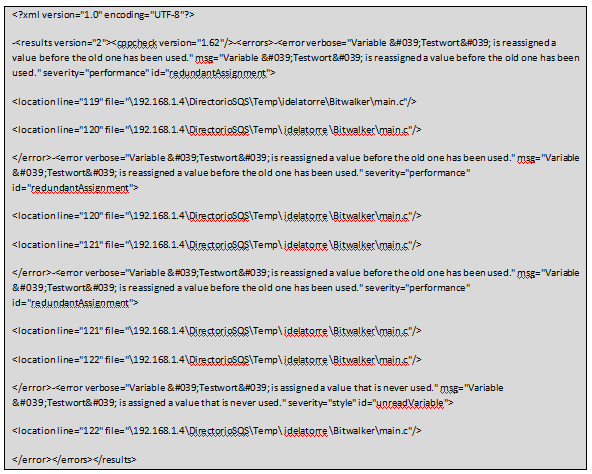
\includegraphics{./figures/cppcheck.png}
\caption{cppcheck results}
\end{figure}

\section{Testwell CMT++ Results}
\label{sec:halsted}
CMT++, Complexity Measures Tool for C/C++, is an easy-to-use code metrics tool for C and C++ languages. Also assembly code, either inlined in a C/C++ source file or separate assembly file, can be measured.

Based on the static properties of the program code CMT++ gives estimates how error prone the program sorce code is due to its complexity, how long it will take to understand the code, what the logical volume of the code is, how much code you have: physical lines, comment lines, program lines, statements, etc

CMT++ helps to estimate the overall maintainability of the code base and easily locate the complex parts of it. 

In this case CMT++ is used to calculate:
\begin{itemize}
\item Basic code complexity metrics
\begin{itemize}
\item McCabe's cyclomatic number
\item Halstead's metrics
\item Lines of code metrics
\item Some other metrics like: number of semicolons, number of function parameter, depth of control structure nesting
\end{itemize}
\item Maintainability Index
\end{itemize}

\subsection{Complexity Metrics}
\subsubsection{Program Size Metrics}
As it was mentioned in \ref{sec:sizem} the number of lines and the Halstead metrics can be used to determine the program size.
\begin{description}
\item \textbf{Number of lines}

The lines of code measures are the most traditional measures used to quantify software complexity. They are simple, easy to count, and very easy to understand. However, they do not take into account the intelligence content and the layout of the code.

CMT++ calculates the following lines-of-code metrics:
\begin{itemize}
\item LOCphy: number of physical lines
\item LOCbl: number of blank lines (a blank line inside a comment block is considered to be a comment line)
\item LOCpro: number of program lines (declarations, definitions, directives, and code)
\item LOCcom: number of comment lines
\end{itemize}

Following the analysis conducted within the tool, the tables below summarizes the results:

\begin{longtable}{||p{.475\textwidth}|p{.115\textwidth}|p{.115\textwidth}|p{.115\textwidth}|p{.115\textwidth}||}
  \caption{Lines of Code Metrics per file}\\
    \hline\hline
    \textbf{File} &\textbf{LOCphy} & \textbf{LOCpro} & \textbf{LOCcom} & \textbf{LOCbl}\\
    \hline\hline
    \endhead
    \hline\hline
    \endfoot
    Bitwalker.c & 109 & 58 & 33 & 23
    \\
    \hline
   \end{longtable}
   
\begin{longtable}{||p{.475\textwidth}|p{.115\textwidth}|p{.115\textwidth}|p{.115\textwidth}|p{.115\textwidth}||}
  \caption{Lines of Code Metrics per functions}\\
    \hline\hline
    \textbf{Function} &\textbf{LOCphy} & \textbf{LOCpro} & \textbf{LOCcom} & \textbf{LOCbl}\\
    \hline\hline
    \endhead
    \hline\hline
    \endfoot
    Bitwalker\_Peek & 20 & 13 & 5 & 4
    \\
    \hline
    Bitwalker\_Poke & 24 & 17 & 6 & 4
    \\
    \hline
    Bitwalker\_IncrementalWalker\_Init & 6 & 6 & 0 & 0
    \\
    \hline
    Bitwalker\_IncrementalWalker\_Peek\_Next & 7 & 6 & 1 & 0
    \\
    \hline
    Bitwalker\_IncrementalWalker\_Peek\_Finish & 4 & 4 & 0 & 0
    \\
    \hline
    Bitwalker\_IncrementalWalker\_Poke\_Next & 7 & 6 & 1 & 0
    \\
    \hline
    Bitwalker\_IncrementalWalker\_Poke\_Finish & 4 & 4 & 0 & 0
    \\
    \hline
   \end{longtable}

\item \textbf{Halstead metrics}

Halstead complexity metrics were developed by the late Maurice Halstead as a mean of determining a quantitative measure of complexity directly from the operators and operands in the module to measure a program module's complexity directly from source code.

Halstead's metrics are based on interpreting the source code as a sequence of tokens and classifying each token to be an operator or an operand. There are based on four basic measures:
\begin{itemize}
\item number of unique (distinct) operators ($n_1$)
\item number of unique (distinct) operands ($n_2$)
\item total number of operators ($N_1$)
\item total number of operands ($N_2$).
\end{itemize}

Taking into account these measures the following metrics will be obtained:
\begin{itemize}
\item Program Vocabulary: $n = n_1 + n_2$
\item Program Length: $N = N_1 + N_2$
\item Program Difficulty: $D = ( n_1 / 2 ) * ( N_2 / n_2 )$
\item Program Volume: $V = N * log_2 (n)$
\item Program Length: L = 1/V
\item Effort to implement: E = V * D
\item Time to implement: T = E / 18
\item Number of delivered bugs: $B = (E^{2/3}) / 3000$
\end{itemize}

So Halstead metrics provide several metrics that focus on different aspects of software complexity. Furthermore, they allow the estimation of development and testing times (with parameter L*V), and difficulty of understanding (with parameter E). 

Software complexity is usually analyzed with the indicators L, V and E due to:
\begin{itemize}
\item the volume is intended being a more accurate measure of the difficulty of understanding a program, taking into account not only its length but also the vocabulary. Halstead's volume (V) describes the size of the implementation of an algorithm.
\item the program level gives an idea of ​​the level of detail that it has been encoded
\item effort can be used as a measure of program clarity since the effort required to produce a piece of software is primarily related to the difficulty to understand and implement it.
\end{itemize}

In the tables below are presented the results obtained per file and per function:

\begin{longtable}{||p{.475\textwidth}|p{.070\textwidth}|p{.060\textwidth}|p{.060\textwidth}|p{.060\textwidth}|p{.060\textwidth}|p{.060\textwidth}|p{.060\textwidth}||}
  \caption{Halstead metrics 1 per file}\\
    \hline\hline
    \textbf{File} &\textbf{L} & \textbf{n} & \textbf{$n_1$} & \textbf{$n_2$} & \textbf{N} & \textbf{$N_1$} & \textbf{$N_2$}\\
    \hline\hline
    \endhead
    \hline\hline
    \endfoot
    Bitwalker.c & 0.014 & 72 & 31 & 41 & 378 & 185 & 193
    \\
    \hline
   \end{longtable}
   
\begin{longtable}{||p{.475\textwidth}|p{.070\textwidth}|p{.125\textwidth}|p{.085\textwidth}|p{.075\textwidth}|p{.090\textwidth}||}
  \caption{Halstead metrics 2 per file}\\
    \hline\hline
    \textbf{File} &\textbf{B} & \textbf{E} & \textbf{T} & \textbf{D} & \textbf{V}\\
    \hline\hline
    \endhead
    \hline\hline
    \endfoot
    Bitwalker.c & 1.024 & 170167.578 & 02:37:33 & 72.963 & 2332.232 
    \\
    \hline
   \end{longtable}
   
\begin{longtable}{||p{.475\textwidth}|p{.070\textwidth}|p{.060\textwidth}|p{.060\textwidth}|p{.060\textwidth}|p{.060\textwidth}|p{.060\textwidth}|p{.060\textwidth}||}
  \caption{Halstead metrics 1 per function}\\
    \hline\hline
    \textbf{Function} &\textbf{L} & \textbf{n} & \textbf{$n_1$} & \textbf{$n_2$} & \textbf{N} & \textbf{$N_1$} & \textbf{$N_2$}\\
    \hline\hline
    \endhead
    \hline\hline
    \endfoot
    Bitwalker\_Peek & 0.041 & 35 & 18 & 17 & 89 & 43 & 46
    \\
    \hline
    Bitwalker\_Poke & 0.028 & 42 & 23 & 19 & 120 & 62 & 58
    \\
    \hline
    Bitwalker\_IncrementalWalker\_Init & 0.143 & 20 & 8 & 12 & 37 & 16 & 21
    \\
    \hline
    Bitwalker\_IncrementalWalker\_Peek\_Next & 0.116 & 20 & 9 & 11 & 39 & 18 & 21
    \\
    \hline
    Bitwalker\_IncrementalWalker\_Peek\_Finish & 0.278 & 11 & 6 & 5 & 12 & 6 & 6
    \\
    \hline
    Bitwalker\_IncrementalWalker\_Poke\_Next & 0.111 & 21 & 9 & 12 & 44 & 20 & 24
    \\
    \hline
    Bitwalker\_IncrementalWalker\_Poke\_Finish & 0.278 & 11 & 6 & 5 & 12 & 6 & 6
    \\
    \hline
   \end{longtable}
   
\begin{longtable}{||p{.475\textwidth}|p{.070\textwidth}|p{.1\textwidth}|p{.085\textwidth}|p{.075\textwidth}|p{.080\textwidth}||}
  \caption{Halstead metrics 2 per function}\\
    \hline\hline
    \textbf{Function} &\textbf{B} & \textbf{E} & \textbf{T} & \textbf{D} & \textbf{V}\\
    \hline\hline
    \endhead
    \hline\hline
    \endfoot
    Bitwalker\_Peek & 0.166 & 11117.269 & 00:10:17 & 24.353 & 456.506 
    \\
    \hline
    Bitwalker\_Poke & 0.267 & 22715.846 & 00:21:01 & 35.105 & 647.078 
    \\
    \hline
    Bitwalker\_IncrementalWalker\_Init & 0.036 & 1119.379 & 00:01:02 & 7.000 & 159.911 
    \\
    \hline
    Bitwalker\_IncrementalWalker\_Peek\_Next & 0.043 & 1448.042 & 00:01:20 & 8.591 & 168.555 
    \\
    \hline
    Bitwalker\_IncrementalWalker\_Peek\_Finish & 0.009 & 149.447 & 00:00:08 & 3.600 & 41.513 
    \\
    \hline
    Bitwalker\_IncrementalWalker\_Poke\_Next & 0.048 & 1739.358 & 00:01:36 & 9.000 & 193.262 
    \\
    \hline
    Bitwalker\_IncrementalWalker\_Poke\_Finish & 0.009 & 149.447 & 00:00:08 & 3.600 & 41.513 
    \\
    \hline
   \end{longtable}

\end{description}

The volume of a function should be at least 20 and at most 1000. The volume of a parameter less one-line function that is not empty; is about 20. A volume greater than 1000 tells that the function probably does too many things.

The volume of a file should be at least 100 and at most 8000. These limits are based on volumes measured for files whose LOCpro and v(G) are near their recommended limits. The limits of volume can be used for double-checking.

Halstead's delivered bugs (B) is an estimate for the number of errors in the implementation.
Delivered bugs in a file should be less than 2. 
Experiences have shown that, when programming with C or C++, a source file almost always contains more errors than B suggests. The number of defects tends to grow more rapidly than B.

By analyzing the results, one can observe that all the Halstead metrics obtained in relation to functions and file are inside the recommendations.


\subsubsection{Control Flow Metrics}
\begin{longtable}{||p{.475\textwidth}|p{.075\textwidth}||}
  \caption{McCabe Cyclomatic Complexity}\\
    \hline\hline
    \textbf{Function} &\textbf{ECC}\\
    \hline\hline
    \endhead
    \hline\hline
    \endfoot
    Bitwalker\_Peek & 3  
    \\
    \hline
    Bitwalker\_Poke & 5  
    \\
    \hline
    Bitwalker\_IncrementalWalker\_Init & 1
    \\
    \hline
    Bitwalker\_IncrementalWalker\_Peek\_Next & 1  
    \\
    \hline
    Bitwalker\_IncrementalWalker\_Peek\_Finish & 1  
    \\
    \hline
    Bitwalker\_IncrementalWalker\_Poke\_Next & 1  
    \\
    \hline
    Bitwalker\_IncrementalWalker\_Poke\_Finish & 1  
    \\
    \hline
   \end{longtable}

As a first conclusion, taking into account the reference table shown in Section \ref{sec:cyclo} the values from the above table indicate a low risk functions and the matching with the results obtained with the previous tools.

\subsection{Maintainability Index}
Maintainability Index (MI) is a single-number value for estimating the relative maintainability of the code. It was designed at the University of Idaho in the 1990s \citep{MI_idaho}

Maintainability Index is calculated with certain formulae from lines-of-code measures, McCabe measure and Halstead measures.

Actually there are three measures:
\begin{itemize}
\item MIwoc: Maintainability Index without comments
\item MIcw: Maintainability Index comment weight
\item MI: Maintainability Index = MIwoc + MIcw
\end{itemize}

The general formulae for MI are the following \citep{MI_IEEE}:

MIwoc = 171 - 5.2 * ln(aveV) -0.23 * aveG -16.2 * ln(aveLOC)

MIcw = 50 * sin(sqrt(2.4 * perCM))

MI = MIwoc + MIcw

where:
\begin{itemize}
\item aveV = average Halstead Volume per Module
\item aveG = average extended cyclomatic complexity per Module
\item aveLOC = average count of lines per Module
\item perCM = average percent of lines of comments per Module
\end{itemize}

\begin{longtable}{||p{.475\textwidth}|p{.075\textwidth}|p{.070\textwidth}|p{.070\textwidth}||}
  \caption{Maintainability Index}\\
    \hline\hline
    \textbf{Function} &\textbf{MIwoc} & \textbf{MIcw} & \textbf{MI}\\
    \hline\hline
    \endhead
    \hline\hline
    \endfoot
    Bitwalker\_Peek & 90 & 35 & 125 
    \\
    \hline
    Bitwalker\_Poke & 85 & 35 & 120 
    \\
    \hline
    Bitwalker\_IncrementalWalker\_Init & 115 & 0 & 115  
    \\
    \hline
    Bitwalker\_IncrementalWalker\_Peek\_Next & 113 & 28 & 140  
    \\
    \hline
    Bitwalker\_IncrementalWalker\_Peek\_Finish & 129 & 0 & 129  
    \\
    \hline
    Bitwalker\_IncrementalWalker\_Poke\_Next & 112 & 28 & 140  
    \\
    \hline
    Bitwalker\_IncrementalWalker\_Poke\_Finish & 129 & 0 & 129  
    \\
    \hline
   \end{longtable}

After calculating the Maintainability Index the maintainability involved can be determined using the following reference table:

{\footnotesize\sffamily\centering
  \begin{longtable}{||p{.15\textwidth}|p{.40\textwidth}||}
  \caption{Maintainability Index Reference table}\\
    \hline\hline
    \textbf{Maintainability Index} & \textbf{Maintainability Evaluation} \\
    \hline\hline
    \endhead
    \hline\hline
    \endfoot
    \textbf{85 and more}
& good maintainability
    \\
    \hline
    \textbf{65-85}
& moderate maintainability
    \\
    \hline
    \textbf{< 65}
& difficult to maintain
with really bad pieces of code (big, uncommented, unstructured) the MI value can be even negative
    \\
    \hline
\end{longtable}}

As a first conclusion, the values from the tables above indicate the functions and file have a good maintanability.

\section{MISRA and Mü8004 Rules Comparation}
This section analyses the requirements designed in MISRA-C : 2004 standard and Mü8004 standard and makes a comparison between rules they might have in common and describes the most important features of the ones they don’t have in common. 

\begin{center}
\textsc{\underline{ENVIRONMENT:}}
\end{center}

%% Debut FRR
\paragraph{MISRA –C Environment Rule 1.1}
MISRA-C Rule 1.1 All code shall conform to ISO/IEC 9899:1990
“Programming languages — C”, amended and corrected by
ISO/IEC 9899/COR1:1995, ISO/IEC 9899/AMD1:1995, and
ISO/IEC 9899/COR2:1996.

This rule is not included in Mü8004 standard. It never mentions which version of C is applied.

\paragraph{MISRA –C Environment Rule 1.2}
MISRA-C Rule 1.2 No reliance shall be placed on undefined or unspecified
behaviour.

This rule is not included in Mü8004 standard. No requirement on behaviour is specified
%% Fin FRR

\paragraph{MISRA –C Environment Rule 1.3}
MISRA-C Rule 1.3 Description: If a module is to be implemented in a language other than C, or compiled on a different C compiler, then it is essential to ensure that the module will integrate correctly with other modules.

This rule is not included in Mü8004 standard. Mü8004 standard establishes in rule 0.2.22 that it is not allowed to change the programming language inside a program module, but not between different modules.

\paragraph{MISRA –C Environment Rule 1.4}
MISRA-C Rule 1.4 Description: The compiler/linker shall be checked to ensure that 31 character significance and case sensitive are supported for external identifiers. If the compiler/linker is not capable of meeting this limit, then use the limit of the compiler.

This rule is not included in Mü8004 standard, although in 0.2.9 rule it is referred that names and identifiers must be chosen in a way that differs significantly in the first 31 positions. This rule should be added.

\paragraph{MISRA –C Environment Rule 1.5}
MISRA-C Rule 1.5 Description: Floating-point implementations should comply with a defined floating-point standard.

This rule is not included in Mü8004 standard and it would be useful adding it to overcome a wide range of problems associated with the use of floating-point arithmetics.

\begin{center}
\textsc{\underline{LANGUAGE EXTENSION:}}
\end{center}

\paragraph{MISRA –C Language extensions 2.1}
MISRA-C Rule 2.1 Description: Where assembly language instructions are required it is recommended that they be encapsulated and isolated in either (a) assembler functions, (b) functions or (c) macros.

This rule is included in Mü8004 Rule 0.2.22, as it establishes that assembler implemented subroutines can be called from C and vice versa. It would be useful to point out that assembler language should not be embedded in normal code.

\paragraph{MISRA –C Language extensions 2.2}
MISRA-C Rule 2.2 Description: Source code shall only use /*…*/ style comments.

This is less restrictive in Mü8004 standard, as // comments are allowed in Mü8004 Rule 0.2.8 if it is supported by compiler. This is correctly focused as this way consistency is not in danger.

\paragraph{MISRA –C Language extensions 2.3}
MISRA-C Rule 2.2 Description: The character sequence /* shall not be used within a comment.

This rule is included in Mü8004 Rule 0.2.8, as it establishes that comments must not be nested. This is an important requirement whose omission would cause critical errors otherwise.

\paragraph{MISRA –C Language extensions 2.4}
MISRA-C Rule 2.4 Description: Sections of code should not be “commented out”

This rule is not included in Mü8004 standard. It would be useful to use conditional compilation (\#if or \#ifdef) for sections of source code not to be compiled, as start and end comment markers for this purpose is dangerous because C does not support nested comments.

%%% debut FRR
\begin{center}
\textsc{\underline{CHARACTER SETS:}}
\end{center}

\paragraph{MISRA –C Character sets 4.1}
MISRA-C Rule 4.1 Only those escape sequences that are defined in the ISO C
standard shall be used.

Mü8004 standard does not include this rule. This rules is useful for code portabiliy.
 
\paragraph{MISRA –C Character sets 4.2}
MISRA-C Rule 4.2 Trigraphs shall not be used


Mü8004 standard does not include this rule. This rules is useful for code understanding. This rule should be mandatory.

%% Fin FRR

\begin{center}
\textsc{\underline{IDENTIFIERS:}}
\end{center}

\paragraph{MISRA –C Identifiers 5.1}
MISRA-C Rule 5.1 Description: Identifiers (internal and external) shall not rely on the significance of more than 31 characters.

This rule is included in Mü8004 Rule 0.2.9, as it establishes that names and identifiers must be chosen in a way that they differ significantly in the first 31 positions.

\paragraph{MISRA –C Identifiers 5.2}
MISRA-C Rule 5.2 Description: Identifiers in an inner scope shall not use the same name as an identifier in an outer scope, and therefore hide that identifier.

This rule is not included in Mü8004 standard, but it would be useful adding it to avoid confusion between identifiers in the code.


\paragraph{MISRA –C Identifiers 5.3}
MISRA-C Rule 5.3 Description: A typedef name shall be a unique identifier.

This rule is not included in Mü8004 standard, but it would be useful adding it to avoid the reuse these names within a program.


\paragraph{MISRA –C Identifiers 5.4}
MISRA-C Rule 5.4 Description: A tag name shall be a unique identifier.

This rule is not included in Mü8004 standard. Although Mü8004 Rule 0.2.9 establishes that same variables should not serve different purposes and it would be useful to avoid the reuse of names within a program for same purposes. This would be useful adding it to avoid confusion.


\paragraph{MISRA –C Identifiers 5.5}
MISRA-C Rule 5.5 Description: No object or function identifier with static storage duration should be reused.

This rule is not included in Mü8004 standard. It would be useful adding it because the possibility exists for the user to incorrectly associate unrelated variables with the same name.

\paragraph{MISRA –C Identifiers 5.6}
MISRA-C Rule 5.6 Description: No identifier in one name space should have the same spelling as an identifier in another name space, with the exception of structure member and union member names.

This rule is not included in Mü8004 standard. It extends the avoidance of using same names for same or different purposes. It will not be applied in the project. 

\paragraph{MISRA –C Identifiers 5.7}
MISRA-C Rule 5.7 Description: No identifier name should be reused (across any files in the system).

This rule is not included in Mü8004 standard. It incorporates the Rules 5.2, 5.3, 5.4, 5.5 and 5.6. It would be an extremely severe requirement to avoid confusion between names.

\paragraph{Mü8004 Identifiers 0.2.9}
Some points of this section, as the following ones, are very important to avoid confusion between names and are not included in Identifiers section in MISRA-C standard:
\begin{itemize}
\item Uppercase and lowercase letters, numbers from 0 to 9, and the sign \$ and \_ are allowed for defining names. ‘\_’ must not be the first character
\item Identifiers that differ only in uppercase/lowercase characters must not have different meaning
\item Identifiers for macros shall be written in uppercase letter
\end{itemize}

\begin{center}
\textsc{\underline{TYPES:}}
\end{center}

\paragraph{MISRA –C Types 6.1}
MISRA-C Rule 6.1 Description: The plain char type shall be used only for the storage and use of character values

This rule is not included in Mü8004 standard. This rule could be useful to set the restriction in the work with this type of data.

\paragraph{MISRA –C Types 6.2}
MISRA-C Rule 6.2 Description: signed and unsigned char type shall be used only for the storage and use of numeric values. Plain char type shall be used for character data.

This rule is not included in Mü8004 standard. This rule could be useful to make a difference between the work with numeric and character data.

\paragraph{MISRA –C Types 6.3}
MISRA-C Rule 6.3 Description: Typedefs that indicate size and signedness should be used in place of the basic numerical types

Mü8004 standard does not show how to use typedef with different data types. However, it shows in Rule 0.2.6 that float and double data types are not supported. This could be a drawback for the precision of variables and operations between them.

\paragraph{MISRA –C Types 6.4}
MISRA-C Rule 6.4 Description: Bit fields shall only be defined to be of type unsigned int or signed int.

This rule is not included in Mü8004 standard, although Mü8004 Rule 0.2.6 establishes that bitfields are permitted. This rule could be useful for the correctness in the work with bitfields.

\paragraph{MISRA –C Types 6.5}
MISRA-C Rule 6.5 Description: Bit fields of signed type shall be at least 2 bits long.

This rule is not included in Mü8004 standard

\begin{center}
\textsc{\underline{CONSTANTS:}}
\end{center}

\paragraph{MISRA –C Types 7.1}
MISRA-C Rule 7.1 Description: Octal constants (other than zero) and octal escape sequences shall not be used

This rule is not included in Mü8004 standard for the definition of constants. Although it defines how to create constants using “const” keyword, it could be interesting not to mix constants and octal, because of potential errors when working with fixed length constants

\paragraph{Mü8004 – 0.2.10 Constants}
Mü8004 – 0.2.10 Constants Rule: Although MISRA-C adds 7.1 Rule that describes the work with octal constants in the standard, Mü8004 - 0.2.10 Constants rule specifies better which is the way to define constants of different type, and the way to use them along the code.

\begin{center}
\textsc{\underline{DECLARATIONS AND DEFINITIONS:}}
\end{center}

\paragraph{MISRA –C Types 8.1}
MISRA-C Rule 7.1 Description: Functions shall have prototype declarations and the prototype shall be visible at both the function definition and call

Mü8004 standard includes at Rule 0.2.15 that function prototypes shall be used for every function whenever the compiler supports it. It would be useful to set the visibility of prototypes for the integrity of function definitions and calls.

\paragraph{MISRA –C Declarations and Definitions 8.2}
MISRA-C Rule 8.2 Description: Whenever an object or function is declared or defined, its type shall be explicitly stated

Mü8004 standard includes at Rule 0.2.15 that function header have to define the function type.

\paragraph{MISRA –C Declarations and Definitions 8.3}
MISRA-C Rule 8.3 Description: For each function parameter the type given in the declaration and definition shall be identical, and the return types shall also be identical

Mü8004 standard does not include this rule, but this rule should be necessary for the proper operation of the function. 

\paragraph{MISRA –C Declarations and Definitions 8.4}
MISRA-C Rule 8.4 Description: If objects or functions are declared more than once their types shall be compatible

Mü8004 standard does not include this rule. It might be good to add this rule to the proper functioning of the code, even though it would be recommendable not to declare objects or functions more than once in order to reduce the number of mistakes made.

\paragraph{MISRA –C Declarations and Definitions 8.5}
MISRA-C Rule 8.5 Description: There shall be no definitions of objects or functions in a header file

Mü8004 standard does not include this rule.  Although Mü8004 Rule 0.2.5 establishes that function prototypes shall only be used in header files, there is no reference to the definition of objects and functions. To prohibit the definition of objects and functions in the header file would be a good programming rule.

\paragraph{MISRA –C Declarations and Definitions 8.6}
MISRA-C Rule 8.6 Description: Functions shall be declared at file scope

There is a restriction in Mü8004 standard Rule 0.2.5 when declaring functions at file scope, because it establishes that function prototypes shall only be used in header files.

\paragraph{MISRA –C Declarations and Definitions 8.7}
MISRA-C Rule 8.7 Description: Objects shall be defined at block scope if they are only accessed from within a single function

Mü8004 standard Rule 0.2.14 establishes that global definitions of structures shall be defined in header files. It would be interesting to add MISRA-C Rule 8.7 for objects that are only used in functions or in block scope.  

\paragraph{MISRA –C Declarations and Definitions 8.8}
MISRA-C Rule 8.8 Description: An external object or function shall be declared in one and only one (external) file

This rule can be added to Mü8004 standard to improve 0.2.14 Rule, as it defines that global definition of structures shall be defined in header files

\paragraph{MISRA –C Declarations and Definitions 8.9}
MISRA-C Rule 8.9 Description: An identifier with external linkage shall have exactly one external definition

Mü8004 does not include this rule. It is necessary to add this rule to fix the work with extern parameter.

\paragraph{MISRA –C Declarations and Definitions 8.10, 8.11}
MISRA-C Rule 8.10 Description: All declarations and definitions of objects or functions at file scope shall have internal linkage unless external linkage is required

MISRA-C Rule8.11 Description: The static storage class specifier shall be used in definitions and declarations of objects and functions that have internal linkage

Mü8004 does not include these rules. It would be useful to avoid confusion between objects with internal scope and objects with external scope.

\paragraph{MISRA –C Declarations and Definitions 8.12}
MISRA-C Rule 8.12 Description: When an array is declared with external linkage, its size shall be stated explicitly or defined implicitly by initialization 

Mü8004 does not include this rule. It could be interesting to add this rule to Mü8004 standard to establish the work with arrays when they are declared with external linkage.


\begin{center}
\textsc{\underline{INITIALIZATION:}}
\end{center}

\paragraph{MISRA –C Initialization 9.1}
MISRA-C Rule 9.1 Description: All automatic variables shall have been assigned a value before being used 

Mü8004 standard includes at Rule 0.2.12 that all variables and fields shall be initialized before they are used the first time.

\paragraph{MISRA –C Initialization 9.2}
MISRA-C Rule 9.2 Description: Braces shall be used to indicate and match the structure in the non-zero initialization of arrays and structures

The use of braces is included in Mü8004 standard Rule 0.2.6, as it establishes that for clearness, the initialization shall be put in curly brackets.

\paragraph{MISRA –C Initialization 9.3}
MISRA-C Rule 9.3 Description: In an enumerator list, the “=” construct shall not be used to explicitly initialize members other than the first, unless all items are explicitly initialized

Mü8004 does not include this rule. It is necessary to avoid making mistakes when initializing enumerators.

%% Debut FRR
\begin{center}
\textsc{\underline{CONVERSIONS:}}
\end{center}

\paragraph{MISRA -C Conversions 10.1}
MISRA-C Rule 10.1 Description: The value of an expression of integer type shall not be implicitly
converted to a different underlying type if:\\
(a)it is not a conversion to a wider integer type of the same
signedness, or \\
(b)the expression is complex, or \\
(c)the expression is not constant and is a function argument, or \\
(d)the expression is not constant and is a return expression

Mü8004 includes this rule. It is a precision of the third phrase of the chapter 0.2.18.

\paragraph{MISRA -C Conversions 10.2}
MISRA-C Rule 10.2 Description: The value of an expression of floating type shall not be implicitly
converted to a different type if:\\
(a) it is not a conversion to a wider floating type, or\\
(b) the expression is complex, or\\
(c) the expression is a function argument, or\\
(d) the expression is a return expression

Mü8004 includes this rule. It is a precision of the thrid phrase of the chapter 0.2.18.

\paragraph{MISRA -C Conversions 10.3}
MISRA-C Rule 10.3 Description: The value of a complex expression of integer type shall only be
cast to a type of the same signedness that is no wider than the
underlying type of the expression.

Mü8004 includes this rule. It is a precision of the third phrase of chapter 0.2.18.

\paragraph{MISRA -C Conversions 10.4}
MISRA-C Rule 10.4 Description: The value of a complex expression of floating type shall only be cast to a floating type that is narrower or of the same size.

Mü8004 includes this rule. It is a precision of the third phrase of the chapter 0.2.18.

\paragraph{MISRA -C Conversions 10.5}
MISRA-C Rule 10.4 Description: If the bitwise operators
\~{} and $<<$ are applied to an operand of underlying type
unsigned char or unsigned short, the result shall
be immediately cast to the underlying type of the operand.

Mü8004 does not include this rule. This operators in this small type then it is a source bug. When type forcing allow the good comportement.

\paragraph{MISRA -C Conversions 10.6}
MISRA-C Rule 10.6 Description: An “U” suffix shall be applied to all constants of unsigned type.

Mü8004 does not include this rule. This rule is for the maintenability and code review.

\paragraph{MISRA -C Conversions 11.1}
MISRA-C Rule 11.1 Description: Conversions shall not be performed between a pointer to a function and any type other than an integral type.

Mü8004 does not include this rule. If this rule was not respected, the code has an undefined behavior. This rule must be mandatory. In addition, the code becomes independent of the compiler.

\paragraph{MISRA -C Conversions 11.2}
MISRA-C Rule 11.2 Description: Conversions shall not be performed between a pointer to object and any type other than an integral type, another pointer to object type or a pointer to void.

Mü8004 does not include this rule. This rule is for the cast system is determinist. And this rules indicates which does not mix pointer and object.

\paragraph{MISRA -C Conversions 11.3}
MISRA-C Rule 11.3 Description: A cast should not be performed between a pointer type and an integral type. 

Mü8004 does not include this rule. This rule is used for not mixing data and pointer. These two objects are different.

\paragraph{MISRA -C Conversions 11.4}
MISRA-C Rule 11.4 Description: A cast should not be performed between a pointer to object type and a different pointer to object type.

Mü8004 does not include this rule. This rule is used for not mix different pointer types for data alignement. This rule prevents safety issues that may
occur if misaligned pointers are used.

\paragraph{MISRA -C Conversions 11.5}
MISRA-C Rule 11.5 Description: A cast shall not be performed that removes any {\it const} or {\it volatile} qualification from the type addressed by a pointer.

Mü8004 does not include this rule. This rule is used for not modified a constant data or a volatile. This rule prevents safety issues that may occur if 
writing to a {\it const} location, or accessing a {\it volatile} location
without proper qualification.

%% end FRR

\begin{center}
\textsc{\underline{EXPRESSIONS:}}
\end{center}

\paragraph{MISRA –C Expressions 12.1}
MISRA-C Rule 12.1 Description: Limited dependence should be placed on C’s operator precedence rules in expressions

Mü8004 does not include this rule. This could be a good advisory rule for the developer that has to be careful with made mistakes because of precedence rule of C. Parentheses should be used to reduce mistakes.

\paragraph{MISRA –C Expressions 12.2}
MISRA-C Rule 12.2 Description: The value of an expression shall be the same under any order of evaluation that the standard permits

Mü8004 standard makes reference to the importance of the influence of evaluation order in expressions.  That’s why Mü8004 Rule 0.2.13 establishes that assignments inside expressions are forbidden and Mü8004 Rule12.2 establishes that post increment and post decrement operators are only allowed if they are placed in a separate expression. However, an advice should be made to the influence of access order in expressions where functions calls, access to volatile objects… are used.

\paragraph{MISRA –C Expressions 12.3}
MISRA-C Rule 12.3 Description: The sizeof operator shall not be used on expressions that contain side effects

Mü8004 Rule 0.2.4 establishes that sizeof operator must not be used after \#if. This operator cannot be used to evaluate an expression. It shall only be applied to an operand which is a type or object.

\paragraph{MISRA –C Expressions 12.4}
MISRA-C Rule 12.4 Description: The right-hand operand of a logical \&\& or || operator shall not contain side effects

Mü8004 standard does not include this rule. This could be a good rule for the developer that has to be careful with side effects when working with these operators.

\paragraph{MISRA –C Expressions 12.5}
MISRA-C Rule 12.5 Description: The operands of a logical \&\& or || shall be primary-expressions
Mü8004 standard does not include this rule. This could be a good rule for both readability of code and for ensuring that the behavior is as the programmer intended.

\paragraph{MISRA –C Expressions 12.6}
MISRA-C Rule 12.6 Description: The operands of logical operators (\&\&, || and !) should be effectively Boolean. Expressions that are effectively Boolean should not be used as operands to operators other than (\&\&, ||, !, =, ==, != and ?:)

Mü8004 Rule 0.2.4 establishes the difference between logical operators (\&\&, ||, !, =, ==, != and ?:) and bitwise (\&=, |, \^{}, -, $>>$, $<<$) operators

\paragraph{MISRA –C Expressions 12.7}
MISRA-C Rule 12.7 Description: Bitwise operators shall not be applied to operands whose underlying type is signed

Mü8004 Rule 0.2.4 establishes that bitwise operators and right shift operators shall only be used with unsigned variables.

\paragraph{MISRA –C Expressions 12.8}
MISRA-C Rule 12.8 Description: The right-hand operand of a shift operator shall lie between zero and one less than the width in bits of the underlying type of the left-hand operand

Mü8004 standard does not include this rule. It could be useful to add this rule and others that talk about the limitations in the work with different operands.

\paragraph{MISRA –C Expressions 12.9}
MISRA-C Rule 12.9 Description: The unary minus operator shall not be applied to an expression whose underlying type is unsigned

Mü8004 Rule 0.2.6 explains the problematic of combining signed and unsigned variables in arithmetic operations. However, this should be extended to explain the problems generated when doing operations as applying operators like unary minus to unsigned variables.

\paragraph{MISRA –C Expressions 12.10}
MISRA-C Rule 12.10 Description: The comma operator shall not be used

Mü8004 Rule 0.2.4 establishes that Mü8004 standard does not support the work with comma operator. 

\paragraph{MISRA –C Expressions 12.11}
MISRA-C Rule 12.11 Description: Evaluation of constant unsigned integer expressions should not lead to wrap-around

Mü8004 standard does not include this rule. This could be a helpful rule to avoid the overflow of unsigned integer expressions.

\paragraph{MISRA –C Expressions 12.12}
MISRA-C Rule 12.12 Description: The underlying bit representations of floating-point values shall not be used

Mü8004 standard does not include this rule. This could be an interesting rule to avoid the errors caused by the way floating-point values are stored, in case this data types would be supported by the compiler.

\paragraph{MISRA –C Expressions 12.13}
MISRA-C Rule 12.13 Description: The increment (++) and decrement (-{}-) operators should not be mixed with other operators in an expression

Mü8004 Rule 0.2.4 establishes the restrictions when working with these operators. Post increment and post decrement operators are only allowed if they are placed in a separate expression.


\begin{center}
\textsc{\underline{CONTROL STATEMENT EXPRESSIONS:}}
\end{center}

\paragraph{MISRA –C Control statement expressions 13.1}
MISRA-C Rule 13.1 Description: Assignment operators shall not be used in expressions that yield a Boolean value

Mü8004 Rule 0.2.13 establishes that assignment operators shall not be used inside expressions that are considered to have a Boolean value.

\paragraph{MISRA –C Control statement expressions 13.2}
MISRA-C Rule 13.2 Description: Tests of a value against zero should be made explicit, unless the operand is effectively Boolean

Mü8004 standard does not include this rule. It could be useful to add this rule for the appropriate work with “not equal” operator.

\paragraph{MISRA –C Control statement expressions 13.3}
MISRA-C Rule 13.3 Description: Floating-point expressions shall not be tested for equality or inequality

Mü8004 standard does not include this rule. This could be an interesting rule if floating-point values are allowed.

\paragraph{MISRA –C Control statement expressions 13.4}
MISRA-C Rule 13.4 Description: The controlling expression of a for statement shall not contain any object of floating type

Mü8004 standard does not include this rule. This could be an interesting rule to avoid making mistakes with for statement, if floating-point values are allowed.

\paragraph{MISRA –C Control statement expressions 13.5}
MISRA-C Rule 13.5 Description: The three expressions of a for statement shall be concerned only with loop control

Mü8004 standard does not include this rule. This is a necessary rule that explains how to work correctly with for statement.

\paragraph{MISRA –C Control statement expressions 13.6}
MISRA-C Rule 13.6 Description: Numeric variables being used within a for loop for iteration counting shall not be modified in the body of the loop

Mü8004 standard does not include this rule. This is a basic rule for the correct work of for loop.

\paragraph{MISRA –C Control statement expressions 13.7}
MISRA-C Rule 13.7 Description: Boolean operations whose results are invariant shall not be permitted

Mü8004 standard does not include this rule. This could be a good rule to avoid the propagation of errors in the program due to wrongly implemented Boolean operations.


\begin{center}
\textsc{\underline{CONTROL FLOW:}}
\end{center}

\paragraph{MISRA –C Control flow 14.1}
MISRA-C Rule 14.1 Description: There shall be no unreachable code

Mü8004 standard does not include this rule, but it is a necessary to avoid mistakes due to code that it is never executed.

\paragraph{MISRA –C Control flow 14.2}
MISRA-C Rule 14.2 Description: All non-null statements shall either: (a) have at least one side-effect however executed, or (b) cause control flow to change

Mü8004 standard does not include this rule. This is a necessary rule to avoid making errors when creating statements.

\paragraph{MISRA –C Control flow 14.3}
MISRA-C Rule 14.3 Description: Before preprocessing, a null statement shall only occur on a line by itself; it may be followed by a comment provided that the first character following the null statement is a white-space character

Mü8004 standard does not include this rule. This is a necessary rule if null statements are allowed to be used. However, the safest way would be not to permit embedding null statements in the code. 

\paragraph{MISRA –C Control flow 14.4}
MISRA-C Rule 14.4 Description: The \textit{goto} statement shall not be used

Mü8004 standard does not include this statement in the list of permitted statements.

\paragraph{MISRA –C Control flow 14.5}
MISRA-C Rule 14.5 Description: The \textit{continue} statement shall not be used

Mü8004 Rule 0.2.3 includes this statement in the list of permitted statements, even though it is recommended to avoid working with it, if possible.

\paragraph{MISRA –C Control flow 14.6}
MISRA-C Rule 14.6 Description: For any iteration statement there shall be at most one break statement used for loop termination

Mü8004 Rule 0.2.3 establishes that every case branch must contain a statement and end with break. This rule is in the interest of good structured programming.

\paragraph{MISRA –C Control flow 14.7}
MISRA-C Rule 14.7 Description: A function shall have a single point of exit at the end of the function

Mü8004 Rule 0.2.3 includes this restriction, as it establishes the use, once per function, of the return statement as the exit point of the function. 

\paragraph{MISRA –C Control flow 14.8}
MISRA-C Rule 14.8 Description: The statement forming the body of a \textit{switch, while, do … while} or \textit{for} statement shall be a compound statement.

Mü8004 Rule 0.2.3 establishes that to facilitate the examination, the program shall be structured with brackets and indentation of lines. This rule should be extended to mention specific cases as, \textit{switch, while, do … while} and \textit{for} cases.

\paragraph{MISRA –C Control flow 14.9}
MISRA-C Rule 14.9 Description: An \textit{if} (expression) construct shall be followed by a compound statement. The \textit{else} keyword shall be followed by either a compound statement, or another \textit{if} statement

Mü8004 Rule 0.2.3 defines the construction of \textit{if} expression. However, it is less restrictive as for an \textit{if} expression with a single statement, braces are not required.

\paragraph{MISRA –C Control flow 14.10}
MISRA-C Rule 14.10 Description: All \textit{if … else if} construct shall be terminated with an else clause

Mü8004 Rule 0.2.3 defines the construction of \textit{if} expression. However, it does not establish how it is the work with this advanced structure. 


\begin{center}
\textsc{\underline{SWITCH STATEMENTS:}}
\end{center}

\paragraph{MISRA –C Switch Statement 15.0}
MISRA-C Rule 15.0 Description: The MISRA C \textit{switch} syntax shall be used

Mü8004 Rule 0.2.3 includes, in a less detailed way, how the construction of a \textit{switch} statement is. 

\paragraph{MISRA –C Switch Statement 15.1}
MISRA-C Rule 15.1 Description: A \textit{switch} label shall only be used when the most closely-enclosing compound statement is the body of a \textit{switch} statement

Mü8004 Rule 0.2.3 includes how \textit{switch, case} and \textit{default} labels have to be used in a \textit{switch} statement.

\paragraph{MISRA –C Switch Statement 15.2}
MISRA-C Rule 15.2 Description: An unconditional \textit{break} statement shall terminate every non-empty \textit{switch} clause

Mü8004 Rule 0.2.3 establishes that every case branch in a \textit{switch} statement must contain a statement and end with \textit{break}.

\paragraph{MISRA –C Switch Statement 15.3}
MISRA-C Rule 15.3 Description: The final clause of a \textit{switch} statement shall be the default clause

Mü8004 Rule 0.2.3 establishes that a default case must be defined in a \textit{switch} statement, and that this is the last statement in the \textit{switch} block.

\paragraph{MISRA –C Switch Statement 15.4}
MISRA-C Rule 15.4 Description: A \textit{switch} expression shall not represent a value that is effectively Boolean

Mü8004 standard does not include this rule. It could be a useful rule to know which data types can be used with \textit{switch} statement, and avoid making mistakes when the \textit{switch} statement is 

\paragraph{MISRA –C Switch Statement 15.5}
MISRA-C Rule 15.5 Description: Every \textit{switch} statement shall have at least one \textit{case} clause

Mü8004 standard does not include this rule. It could be useful to add this rule to clarify the necessity of adding at least one case clause in every \textit{switch} statement.

\begin{center}
\textsc{\underline{POINTERS AND ARRAYS:}}
\end{center}

\paragraph{MISRA –C Pointers and Arrays 17.1}
MISRA-C Rule 17.1 Description: Pointer arithmetic shall only be applied to pointers that address an array or array element

Mü8004 standard does not include this rule. This is a necessary rule to determine how pointers arithmetic has to be applied in order to have an expected behaviour.

\paragraph{MISRA –C Pointers and Arrays 17.2}
MISRA-C Rule 17.2 Description: Pointer subtraction shall only be applied to pointers that address elements of the same array

Mü8004 standard does not include this rule. This is a necessary rule if the result we want to get is the number of elements separating the pointers.

\paragraph{MISRA –C Pointers and Arrays 17.3}
MISRA-C Rule 17.3 Description: >, >=, <, <= shall not be applied to pointer types except where they point to the same array

Mü8004 standard does not include this rule. This is a necessary rule if the behavior we want to obtain after the comparison of the pointers it is a well-defined behavior.

\paragraph{MISRA –C Pointers and Arrays 17.4}
MISRA-C Rule 17.4 Description: Array indexing shall be the only allowed form of pointer arithmetic

Mü8004 standard does not include this rule. This rule would help to avoid making mistakes like accessing to invalid memory addresses after manipulation of pointers.

\paragraph{MISRA –C Pointers and Arrays 17.5}
MISRA-C Rule 17.5 Description: The declaration of objects should contain no more than 2 levels of pointer indirection

Mü8004 standard does not include this rule. Although this would not be a required rule, it would help to improve the readability of the code and avoid making mistakes because of the complexity of instructions.

\paragraph{MISRA –C Pointers and Arrays 17.6}
MISRA-C Rule 17.6 Description: The address of an object with automatic storage shall not be assigned to another object that may persist after the first object has ceased to exist

Mü8004 Rule 0.2.17 does include this rule, as it establishes that addresses of auto variables shall only be stored in auto variables of the same visibility. 

\paragraph{Mü8004 – 0.2.17 Pointer}
Mü8004 – 0.2.17 Pointer Rule: Although MISRA-C includes rules about Pointers, it is necessary to establish the limitation of the relation between pointers and the functions, and pointers and the definition of some variables.

\begin{center}
\textsc{\underline{STRUCTURES AND UNIONS:}}
\end{center}

\paragraph{MISRA –C Structures and Unions 18.1}
MISRA-C Rule 18.1 Description: All structure and union types shall be complete at the end of a translation unit

Mü8004 standard does not include this rule. This is a basic rule that shows how the definition of structures has to be made.

\paragraph{MISRA –C Structures and Unions 18.2}
MISRA-C Rule 18.2 Description: An object shall not be assigned to an overlapping object

Mü8004 standard does not include this rule. Although this rule refers to low-level programming, it could be useful in case it is permitted to create two objects having some overlap in memory.

\paragraph{MISRA –C Structures and Unions 18.3}
MISRA-C Rule 18.3 Description: An area of memory shall not be reused for unrelated purposes

Mü8004 standard does not include this rule. This could be an interesting rule to avoid making mistakes by storing unrelated data in the same piece of memory. However, exceptions should be made for requirements of memory efficiency.

\paragraph{MISRA –C Structures and Unions 18.4}
MISRA-C Rule 18.4 Description: Unions shall not be used

Mü8004 Rule 0.2.6 contradicts this rule. Unions could be used in situations in which the use of unions is advisable for an implementation that has to be efficient in terms of memory.


\begin{center}
\textsc{\underline{DOCUMENTATION:}}
\end{center}

\paragraph{MISRA –C Documentation 3.1}
MISRA-C Rule 3.1 Description: All usage of implementation-defined behavior shall be documented

Mü8004 standard does not include this rule. This could be a useful rule to guarantee that the standard’s behavior is completely documented and covered by the defined rules.

\paragraph{MISRA –C Documentation 3.2}
MISRA-C Rule 3.2 Description: The character set and the corresponding encoding shall be documented

Mü8004 standard does not include this rule. As standard’s requirements have to be documented, same thing should be made with encoding of permitted character sets.

\paragraph{MISRA –C Documentation 3.3}
MISRA-C Rule 3.3 Description: The implementation of integer division in the chosen compiler should be determined, documented and taken into account

Mü8004 standard does not include this rule. It should be documented the way arithmetic operations are done, and what are the limitations of operators and the expected behavior.

\paragraph{MISRA –C Documentation 3.4}
MISRA-C Rule 3.4 Description: All uses of \textit{\#pragma} directive shall be documented and explained

Mü8004 standard does not include this rule. Although Mü8004 Rule 0.2.5 establishes that the use of the \textit{\#pragma} command requires a special explanation in the proof of functionality, it doesn’t require documenting its use. 

\paragraph{MISRA –C Documentation 3.5}
MISRA-C Rule 3.5 Description: If it is being relied upon, the implementation defined behavior and packing of bitfields shall be documented

Mü8004 standard does not include this rule. It could be a useful rule to settle how the work with bit fields has to be done. 

\paragraph{MISRA –C Documentation 3.6}
MISRA-C Rule 3.6 Description: All libraries used in production code shall be written to comply with the provisions of this document, and shall have been subject to appropriate validation

Mü8004 standard does not include this rule. It could be a useful rule to document what libraries have been used in the production of the code, or the ones supplied by the compiler.

\paragraph{Mü8004 – 0.2.3 Coding of Basic Structures}
Mü8004 – 0.2.3 Coding of Basic Structures Rule: Although MISRA-standard includes the way of working with basic structures like if-else, switch-case and do-while, Mü8004 standard defines clearly how this structures have to be defined.

\paragraph{Mü8004 – 0.2.4 Operators}
Mü8004 – 0.2.4 Operator Rule: Although MISRA-standard includes explanation for the most important operators, it is helpful to have a general overview of them within a table.

\paragraph{Mü8004 – 0.2.11 Variables}
Mü8004 – 0.2.11 Variables Rule: Mü8004 - 0.2.11 Variables rule explains the correct way of defining variables. Although the content of this rule has been treated in MISRA-C standard, it is appropriate to use a specific section to explain the work with variables.

\paragraph{Mü8004 – 0.2.19 Data References}
Mü8004 – 0.2.19 Data References Rule: Although MISRA-C includes rules about Documentation, it is necessary to make a reference to the documentation of data related and not related to the project planning, and not only to the data and to the libraries used along the code.

\paragraph{Mü8004 – 0.2.20 Cross Reference List}
Mü8004 – 0.2.20 Cross Reference List Rule: MISRA-C doesn’t include the necessity of using cross reference list for the data of the code. It also could be useful to add the characteristics that need to have the development tools used for this purpose.

\paragraph{Mü8004 – 0.2.21 Assembler Coding}
Mü8004 – 0.2.21 Assembler Coding Rule: MISRA-C doesn’t include the necessity of justifying the use of assembler coding. It is helpful to specify that assembler could be useful in time critical programming.

\paragraph{Mü8004 – 0.2.25 Optimization}
Mü8004 – 0.2.25 Optimization Rule: Although MISRA-standard includes the importance of the characteristics of compiler used in the development environment, it is useful to explain the influence of optimization in the compiler.

\section{Conclusions}

Static analysis tools are very good due to the detection of several problem/errors at code level that are usually difficult to detect by manual inspection. Furthermore, they help enforce coding standards and keep code complexity low.

However, these tools sometimes report false positives so it is necessary to review them and decide if they are related with problems or not. Nonetheless, it is recommended to complement the static analysis tools with manual code inspections (not thought of by the original coder) and dynamic analysis.

In order to ensure the correctness of the obtained results mentioned in the previous sections, a comparison of them was executed.

\begin{longtable}{||p{.225\textwidth}|p{.125\textwidth}|p{.125\textwidth}|p{.125\textwidth}|p{.125\textwidth}||}
  \caption{File Size metrics comparation}\\
    \hline\hline
    \endhead
    \hline\hline
    \endfoot
\multicolumn{5}{||l||}{\textbf{Bitwalker.c}}
\\\hline
\ \textbf{Metric} & \textbf{RSM} & \textbf{LocMetric} & \textbf{Understand} & \textbf{CMT++}
\\\hline
\ Total lines: & 109 & \textcolor{red}{110} & 109 & 109
\\\hline
\ Code/program lines: & 58 & 58 & 58 & 58
\\\hline
\ Comment lines: & \textcolor{red}{29} & 28+5 = 33 & 33 & 33 
\\\hline
\ Blank lines: & - & \textcolor{red}{24} & 23 & 23
 \\\hline
\end{longtable}

As a result of this comparison we obtain that between the tools there are some small deviations regarding some code metrics like total lines, comments or blank lines. Thus it was necessary to check how each aspect/metric is defined into each tool.

A manual inspection was done and the source of inconsistency is due to LocMetricss counts the last blank line of the file and RSM tool does not count the blank lines that are inside one commented section.

In addition to code size metrics of file, size code metrics per function were compared.

\begin{longtable}{||p{.225\textwidth}|p{.125\textwidth}|p{.125\textwidth}|p{.125\textwidth}|p{.125\textwidth}||}
  \caption{Functions Size metrics comparation}\\
    \hline\hline
    \endhead
    \hline\hline
    \endfoot
\ \textbf{Metric} & \textbf{RSM} & \textbf{LocMetric} & \textbf{Understand} & \textbf{CMT++}
\\\hline
\multicolumn{5}{||l||}{\textbf{Bitwalker\_Peek}}
\\\hline
\ Total lines: & \textcolor{red}{19} & - & 20 & 20
\\\hline
\ Code/program lines: & \textcolor{red}{12} & - & 13 & 13
\\\hline
\ Comment lines: & 5 & - & 5 & 5 
\\\hline
\ Blank lines: & - & - & 4 & 4
 \\\hline
 \multicolumn{5}{||l||}{\textbf{Bitwalker\_Poke}}
\\\hline
\ Total lines: & \textcolor{red}{23} & - & 24 & 24
\\\hline
\ Code/program lines: & \textcolor{red}{16} & - & 17 & 17
\\\hline
\ Comment lines: & 6 & - & 6 & 6 
\\\hline
\ Blank lines: & - & - & 4 & 4
 \\\hline
 \multicolumn{5}{||l||}{\textbf{Bitwalker\_IncrementalWalker\_Init}}
\\\hline
\ Total lines: & \textcolor{red}{5} & - & 6 & 6
\\\hline
\ Code/program lines: & \textcolor{red}{5} & - & 6 & 6
\\\hline
\ Comment lines: & 0 & - & 0 & 0 
\\\hline
\ Blank lines: & - & - & 0 & 0
 \\\hline
 \multicolumn{5}{||l||}{\textbf{Bitwalker\_IncrementalWalker\_Peek\_Next}}
\\\hline
\ Total lines: & \textcolor{red}{6} & - & 7 & 7
\\\hline
\ Code/program lines: & \textcolor{red}{5} & - & 6 & 6
\\\hline
\ Comment lines: & 1 & - & 1 & 1 
\\\hline
\ Blank lines: & - & - & 0 & 0
 \\\hline
 \multicolumn{5}{||l||}{\textbf{Bitwalker\_IncrementalWalker\_Peek\_Finish}}
\\\hline
\ Total lines: & \textcolor{red}{3} & - & 4 & 4
\\\hline
\ Code/program lines: & \textcolor{red}{3} & - & 4 & 4
\\\hline
\ Comment lines: & 0 & - & 0 & 0 
\\\hline
\ Blank lines: & - & - & 0 & 0
 \\\hline
 \multicolumn{5}{||l||}{\textbf{Bitwalker\_IncrementalWalker\_Poke\_Next}}
\\\hline
\ Total lines: & \textcolor{red}{6} & - & 7 & 7
\\\hline
\ Code/program lines: & \textcolor{red}{5} & - & 6 & 6
\\\hline
\ Comment lines: & 1 & - & 1 & 1 
\\\hline
\ Blank lines: & - & - & 0 & 0
 \\\hline
 \multicolumn{5}{||l||}{\textbf{Bitwalker\_IncrementalWalker\_Poke\_Finish}}
\\\hline
\ Total lines: & \textcolor{red}{3} & - & 4 & 4
\\\hline
\ Code/program lines: & \textcolor{red}{3} & - & 4 & 4
\\\hline
\ Comment lines: & 0 & - & 0 & 0 
\\\hline
\ Blank lines: & - & - & 0 & 0
 \\\hline
\end{longtable}

The total lines and program lines counts produced by some of the tool for the same product differ a little bit. 
The results clearly demonstrate the effects of existing ambiguities in code counting methodology and a variety of interpretations.

McCabe cyclomatic complexity was another complexity metric calculated by different of the selected tools. 

\begin{longtable}{||p{.475\textwidth}|p{.125\textwidth}|p{.125\textwidth}|p{.125\textwidth}||}
  \caption{function Cyclomatic Complexity comparation}\\
    \hline\hline
    \textbf{Function} &\textbf{RSM} & \textbf{Understand} & \textbf{CMT++} \\
    \hline\hline
    \endhead
    \hline\hline
    \endfoot
    Bitwalker\_Peek & 3 & 3 & 3
    \\
    \hline
    Bitwalker\_Poke & 5 & 5 & 5 
    \\
    \hline
    Bitwalker\_IncrementalWalker\_Init & 1 & 1 & 1
    \\
    \hline
    Bitwalker\_IncrementalWalker\_Peek\_Next & 1 & 1 & 1
    \\
    \hline
    Bitwalker\_IncrementalWalker\_Peek\_Finish & 1 & 1 & 1
    \\
    \hline
    Bitwalker\_IncrementalWalker\_Poke\_Next & 1 & 1 & 1
    \\
    \hline
    Bitwalker\_IncrementalWalker\_Poke\_Finish & 1 & 1 & 1
    \\
    \hline
\end{longtable}

According to McCabe a value of 10 is a practical upper limit for the cyclomatic complexity of a given module. When the complexity exceeds this value, it becomes very difficult to prove, understand and modify the module. However, in some circumstances, it may be appropriate to relax the restriction and permit modules with a complexity as high as 15.

Analyzing the cyclomatic complexity metric measured one can observe the low risk of each function and all tools measured it in the same way.

In relation to the MISRA-C rules, as each tool verifies a subset of the rules defined in this standard, the results are different. However, the violations relationed with rules that are included in both RMS and Understand tool have been detected by both tools.

The accepted values for the metrics are defined based on the specific project requirements, project quality criteria or sector best practices. Depending on the metrics required for a project, one or more tools can be used. By this reason a selection of some MISRA-C and other standard to be applied shall be done and each specific violation and quality notice shall be analysed to check the suitability of applied the rule or not. 

Taking into account all the obtained results, we can concluded that:
\begin{itemize}
\item the functions and file have a good maintanability due to the maintainability Index is >85 in both of them
\item the functions have little logic and low risk regarding to the cyclomatic complexity values
\item the functions and file have an appropiate size and inside the recommendations due to line metrics and Halstead metrics.
\item there are some misra-c rules violations and quality notice although these shall be taken into account only in case they are related to the selected ruled to be applied.
\item there are some functions never used
\end{itemize}

In addition to these, as each existing static analysis tool implements different and very specific techniques (code metrics analysis, semantic analysis, context analysis -interactions between multiple functions calls-, creation of new rules, support coding rules/standard rules, ...) to achieve the required assessment or verification objectives, it is recommended to select different static analysis to cover all the commom areas where problems can occur.
\cleardoublepage

\chapter{Conclusions}
\label{sec:conclusions}

\fxfatal{issue 169: As the bitwalker example allows a limited usage of the approach, could you give in conclusion some feedbacks from previous experience ? in which case this approach is efficient to be used ?}

\fxfatal{issue 169: This report presents experiment swith two complementary approaches, is it possible to have in conclusion some comments on which approach is recommended to be used in the openETCS project, on which artifacts and to cover which objectives of VnV ? Then which steps of VnV are expected to cover EN50128 requirements and are not covered by these approaches ?}
\cleardoublepage


\bibliographystyle{unsrt}
\bibliography{bibliography}

\nocite{*}
%===================================================
%Do NOT change anything below this line

\end{document}
